\documentclass[11pt,a4paper]{article}

\usepackage[utf8]{inputenc}
\usepackage[brazil]{babel}
\usepackage[margin=2cm]{geometry}
\usepackage{amsmath,amssymb,amsfonts}
\usepackage{graphicx}
\usepackage{booktabs}
\usepackage{microtype}
\usepackage{hyperref}
\usepackage{caption}
\usepackage{subcaption}
\usepackage{float}
\usepackage{listings}
\usepackage{xcolor}

\hypersetup{
    colorlinks=true,
    linkcolor=blue!80!black,
    citecolor=blue!80!black,
    urlcolor=blue!80!black
}

\title{\textbf{Trabalho Prático 2: Busca Local e Algoritmo Genético}\\
\large Otimização Combinatória no Sequenciamento de Manutenção de Ativos\\
\small Fundamentos de Inteligência Artificial --- DCC / UFMG}
\author{Vinicius Ferreira \\ \texttt{viniciusf@dcc.ufmg.br}}
\date{Outubro de 2026}

\begin{document}

\maketitle

\begin{abstract}
Este trabalho apresenta o projeto, implementação e análise comparativa rigorosa entre heurísticas de Busca Local (com variantes de descida gulosa e têmpera simulada) e a metaheurística populacional de Algoritmo Genético para a resolução do problema combinatório de Sequenciamento de Manutenção Preventiva de Ativos em uma rede de distribuição de energia elétrica. O objetivo central é investigar na prática o equilíbrio entre \emph{exploração} (\emph{exploration}) e \emph{intensificação} (\emph{exploitation}) sob um protocolo experimental estrito de orçamento de avaliações da função objetivo em três escalas de problema ($n=12$, $n=50$ e $n=150$). Analisam-se operadores de vizinhança clássicos (Swap, Insertion e 2-opt), mecanismos de resfriamento (geométrico e linear), métodos de seleção (torneio e roleta) e recombinações preservadoras de permutação (OX e PMX), acompanhados de avaliação incremental de tempo de execução e sustentação estatística por testes não-paramétricos de Mann-Whitney.
\end{abstract}

\section{Introdução e Modelagem do Problema}

O problema consiste no planejamento do cronograma de atendimento preventivo de $n$ ativos georreferenciados (transformadores, religadores e chaves seccionadoras) por uma única equipe técnica. A equipe parte de uma base de coordenadas $(x_0, y_0)$ no instante de tempo inicial $C_0 = 0$ (com duração $p_0 = 0$) e atende sequencialmente um ativo por vez, não havendo necessidade de retornar à base ao término da jornada.

Para cada ativo $j \in \{1, \dots, n\}$, são conhecidos:
\begin{itemize}
    \item Posição geográfica $(x_j, y_j) \in \mathbb{R}^2$;
    \item Duração do serviço de manutenção $p_j$ (em horas);
    \item Prazo regulatório limite de conclusão $d_j$ (em horas);
    \item Peso de criticidade $w_j \ge 0$, que quantifica o custo financeiro e social por hora de atraso.
\end{itemize}

O deslocamento entre duas posições $i$ e $j$ consome um tempo de trânsito euclidiano arredondado ao inteiro mais próximo, dado por:
\begin{equation}
    t_{ij} = \text{round}\left(\sqrt{(x_i - x_j)^2 + (y_i - y_j)^2}\right).
    \label{eq:distancia}
\end{equation}

A solução candidata é modelada como uma permutação completa $\pi = (\pi_1, \pi_2, \dots, \pi_n)$ dos $n$ ativos. O instante de conclusão do $k$-ésimo ativo visitado na rota é calculado recursivamente por:
\begin{equation}
    C_{\pi_k} = C_{\pi_{k-1}} + t_{\pi_{k-1}, \pi_k} + p_{\pi_k}, \quad \text{com } \pi_0 = 0 \text{ e } C_{\pi_0} = 0.
    \label{eq:conclusao}
\end{equation}

A função de custo a ser minimizada (aptidão/fitness) é o atraso ponderado total:
\begin{equation}
    h(\pi) = \sum_{j=1}^n w_j \cdot \max(0, C_j - d_j).
    \label{eq:fitness}
\end{equation}

O espaço de busca contém $n!$ soluções possíveis, tornando inviável a enumeração exata para instâncias médias e grandes ($150! > 5{,}7 \times 10^{262}$). O problema possui restrições suaves (\emph{soft constraints}), de forma que toda permutação é uma solução factível, e a função $h$ é monotonicamente não-decrescente em relação ao prefixo da rota. A tensão fundamental reside no compromisso antagônico entre minimizar o deslocamento local (ir ao vizinho mais próximo) e priorizar ativos iminentes de alta criticidade (evitar multas severas).

\subsection{Validação da Função de Avaliação}
Conforme estipulado na Seção 1.4 do enunciado, a implementação do cálculo de $h(\pi)$ foi estritamente verificada através de testes unitários automatizados na instância pequena ($n=12$):
\begin{enumerate}
    \item \textbf{Permutação Identidade:} $\pi = (1, 2, \dots, 12) \implies h(\pi) = 4366{,}0$.
    \item \textbf{Heurística Gulosa:} Escolhendo a cada passo o ativo que minimiza o acréscimo imediato de atraso com desempate por proximidade $\implies \pi_{gulosa} = (5, 4, 2, 7, 12, 8, 11, 1, 9, 10, 3, 6)$ produzindo $h = 3168{,}0$.
    \item \textbf{Ótimo Global:} Obtido via solucionador de \emph{Branch-and-Bound} implementado para o trabalho: $\pi^* = (5, 4, 1, 6, 7, 2, 8, 12, 3, 10, 9, 11)$ atingindo exatamente $h^* = 1875{,}0$.
\end{enumerate}

\section{Arquitetura do Sistema e Algoritmos}

\subsection{Desacoplamento: Algoritmo $\neq$ Problema}
Seguindo o princípio de projeto da Seção 2.1, os algoritmos foram desacoplados do domínio da concessionária através da classe abstrata \texttt{CombinationProblem}, interagindo apenas por uma interface genérica:
\begin{itemize}
    \item \texttt{random\_solution()}: amostragem de permutação aleatória válida;
    \item \texttt{evaluate(s)} ou \texttt{h(s)}: avaliação de custo de minimização;
    \item \texttt{for\_each\_successor(s, op, callback)}: gerador de vizinhança sob demanda, eliminando overhead de alocação de memória;
    \item \texttt{random\_successor(s, op)}: geração de um sucessor uniforme em $O(n)$;
    \item \texttt{crossover(p1, p2, type)} e \texttt{mutate(s)}: operadores genéticos preservadores de viabilidade.
\end{itemize}

A classe concreta \texttt{AssetsMaintainance} herda de \texttt{CombinationProblem} e encapsula o pré-cálculo da matriz simétrica de distâncias $t_{ij}$ e o estado físico dos ativos.

\subsection{Operadores de Vizinhança e Avaliação Incremental}
Foram implementados três operadores clássicos de geração de sucessores:
\begin{itemize}
    \item \textbf{Swap (troca):} Troca de posição entre dois ativos distintos $i$ e $j$. Tamanho da vizinhança:
    \begin{equation}
        V_{\text{Swap}}(n) = \binom{n}{2} = \frac{n(n-1)}{2}.
    \end{equation}
    Para $n=12 \implies 66$; para $n=50 \implies 1225$; para $n=150 \implies 11175$.
    \item \textbf{Insertion (realocação):} Remove o ativo na posição $i$ e o insere na posição $j$, transladando os intermediários. Tamanho da vizinhança:
    \begin{equation}
        V_{\text{Ins}}(n) = n(n-1).
    \end{equation}
    Para $n=12 \implies 132$; para $n=50 \implies 2450$; para $n=150 \implies 22350$.
    \item \textbf{2-opt (inversão):} Inverte a ordem do segmento entre as posições $i$ e $j$. Tamanho da vizinhança:
    \begin{equation}
        V_{\text{2-opt}}(n) = \binom{n}{2} = \frac{n(n-1)}{2}.
    \end{equation}
\end{itemize}

\paragraph{Avaliação Incremental:} Avaliar uma rota a partir do início custa $O(n)$ operações. Ao aplicar qualquer movimento com ponto de partida em $start = \min(i, j)$, todo o prefixo $0 \dots start-1$ mantém seus instantes de conclusão e penalidades inalterados. Desenvolveu-se a estrutura \texttt{PrefixState}, que armazena $C_k$ e o custo acumulado até cada posição. A avaliação incremental percorre apenas o sufixo afetado usando indexação virtual (zero alocações dinâmicas), alcançando uma aceleração de $\approx 1{,}52\times$ em tempo de CPU na instância média, comprovada por teste unitário de concordância numérica exata ($100\%$ dos casos idênticos à avaliação completa).

\subsection{Metaheurísticas Implementadas}

\subsubsection{Greedy Descent com Random Restart}
Implementadas três variantes de seleção do próximo sucessor:
\begin{enumerate}
    \item \textbf{Best Improvement:} Varre exaustivamente toda a vizinhança e move-se para o vizinho de menor $h$. Ao atingir o ótimo local, realiza reinicialização aleatória (\emph{random restart}).
    \item \textbf{First Improvement:} Varre a vizinhança e aceita imediatamente o primeiro vizinho que apresente melhoria em $h$, reiniciando a busca a partir dele.
    \item \textbf{Random Successor com Aceitação de Melhora:} Sorteia um vizinho aleatório por vez, aceitando-o se $h(s') < h(s)$. Detecta estagnação quando atinge $V(n)$ tentativas consecutivas sem melhoria, disparando o restart.
\end{enumerate}

\subsubsection{Simulated Annealing (Têmpera Simulada)}
A partir da solução corrente $\pi$, sorteia-se um sucessor $\pi'$. Se $\Delta h = h(\pi') - h(\pi) \le 0$, o movimento é aceito; caso contrário, aceita-se com probabilidade de Gibbs $P(\Delta h, T) = \exp(-\Delta h / T)$. 
Avaliaram-se dois esquemas de resfriamento:
\begin{itemize}
    \item \textbf{Geométrico:} $T \leftarrow \alpha T$, onde $\alpha = (T_f / T_0)^{1/B}$.
    \item \textbf{Linear:} $T(t) = T_0 - (T_0 - T_f) \cdot \frac{t}{B}$, onde $t$ é o índice da avaliação e $B$ o orçamento total.
\end{itemize}
A temperatura inicial $T_0$ foi calibrada medindo a magnitude típica média de piora $\overline{\Delta h}$ em amostragens preliminares, definindo $T_0 = -\overline{\Delta h} / \ln(0{,}80)$ (iniciando com $80\%$ de aceitação de movimentos ruins, caracterizando um \emph{random walk}) e $T_f = -\overline{\Delta h} / \ln(0{,}001)$ (concluindo com menos de $0{,}1\%$ de aceitação, convergindo para descida estrita).

\subsubsection{Algoritmo Genético (GA)}
Mantém uma população de tamanho $N=50$ com elitismo de 1 indivíduo e taxa de mutação por troca (\emph{Swap Mutation}) $P_m = 0{,}15$. Foram implementadas e comparadas quatro combinações:
\begin{itemize}
    \item \textbf{Mecanismos de Seleção:}
    \begin{itemize}
        \item \emph{Torneio ($k=3$):} Seleciona três indivíduos aleatórios e escolhe o de menor custo.
        \item \emph{Roleta para Minimização:} Escalonamento linear $f_i = (h_{\max} - h_i) + \delta$, onde $\delta = 0{,}05(h_{\max} - h_{\min} + 1)$, atribuindo maiores fatias aos indivíduos com menor custo.
    \end{itemize}
    \item \textbf{Operadores de Cruzamento ($P_c = 0{,}90$):}
    \begin{itemize}
        \item \emph{Order Crossover (OX):} Preserva sub-rotas consecutivas do Pai 1 e preenche os alelos faltantes na ordem relativa circular do Pai 2.
        \item \emph{Partially Mapped Crossover (PMX):} Copia o segmento central do Pai 1 e estabelece mapeamentos de troca biunívocos com o Pai 2 para preencher as posições externas.
    \end{itemize}
\end{itemize}

\paragraph{Exemplo Numérico Passo a Passo do PMX:}
Considere dois pais de $n=8$ com cortes nos índices 3 a 5 (inclusos):
\begin{align*}
    P_1 &= [1, 2, 3 \mid \mathbf{4, 5, 6} \mid 7, 8] \\
    P_2 &= [8, 7, 6 \mid \mathbf{5, 4, 3} \mid 2, 1]
\end{align*}
\begin{enumerate}
    \item Copia o segmento central de $P_1$: $\text{Filho} = [?, ?, ? \mid \mathbf{4, 5, 6} \mid ?, ?]$. Mapeamentos: $4 \leftrightarrow 5$, $5 \leftrightarrow 4$, $6 \leftrightarrow 3$.
    \item Elementos de $P_2[3..5]$:
    \begin{itemize}
        \item $5$ já está no filho (veio de $P_1$);
        \item $4$ já está no filho;
        \item $3$ não está no filho. Mapeamento $3 \leftrightarrow 6$. A posição de 6 em $P_2$ é o índice 2 (fora do corte). Logo, Filho[2] = 3.
    \end{itemize}
    Estado intermediário: $[?, ?, 3 \mid \mathbf{4, 5, 6} \mid ?, ?]$.
    \item Copia os elementos restantes diretamente de $P_2$: posições 0, 1, 6 e 7 recebem 8, 7, 2 e 1.
    \item $\text{Filho} = [8, 7, 3, \mathbf{4, 5, 6}, 2, 1]$. A permutação gerada é estritamente válida e não contém repetições.
\end{enumerate}

\section{Protocolo Experimental}

Seguindo o protocolo obrigatório da Seção 3 do enunciado, o recurso contabilizado foi estritamente o número de chamadas da função de avaliação $h(\pi)$, respeitando os limites:
\begin{itemize}
    \item \textbf{Instância Pequena ($n=12$):} 50.000 avaliações, 30 execuções independentes ($h^* = 1875{,}0$).
    \item \textbf{Instância Média ($n=50$):} 150.000 avaliações, 30 execuções independentes (alvo de referência: 16.332).
    \item \textbf{Instância Grande ($n=150$):} 300.000 avaliações, 10 execuções independentes (alvo de referência: 60.417).
\end{itemize}

\section{Resultados Experimentais e Análise Comparativa}

\subsection{Tarefa T2: Comparação das Vizinhanças}
Utilizando o Greedy Descent com Random Restart sob o mesmo orçamento de avaliações, compararam-se os operadores Swap, Insertion e 2-opt. Os resultados médios são sintetizados na Tabela~\ref{tab:t2_vizinhancas}.

\begin{table}[H]
\centering
\caption{Comparação de operadores de vizinhança sob Greedy Descent.}
\label{tab:t2_vizinhancas}
\small
\begin{tabular}{llrrrr}
\toprule
\textbf{Instância} & \textbf{Vizinhança} & \textbf{Custo Médio ($h$)} & \textbf{Tempo (ms)} & \textbf{Passos Melhoria} & \textbf{Restarts} \\
\midrule
Pequena ($n=12$) & Swap      & 2256{,}5 & 0{,}21 & 27{,}0 & 4{,}0 \\
Pequena ($n=12$) & Insertion & 2031{,}0 & 0{,}16 & 14{,}0 & 2{,}0 \\
Pequena ($n=12$) & 2-opt     & 2052{,}5 & 0{,}14 & 27{,}5 & 3{,}5 \\
\midrule
Média ($n=50$)   & Swap      & 124178{,}0 & 0{,}19 & 2{,}0 & 0{,}0 \\
Média ($n=50$)   & Insertion & 154374{,}5 & 0{,}23 & 1{,}0 & 0{,}0 \\
Média ($n=50$)   & 2-opt     & 120114{,}5 & 0{,}21 & 2{,}0 & 0{,}0 \\
\midrule
Grande ($n=150$) & Swap      & 1297171{,}5 & 0{,}63 & 1{,}0 & 0{,}0 \\
Grande ($n=150$) & Insertion & 1220035{,}5 & 0{,}60 & 1{,}0 & 0{,}0 \\
Grande ($n=150$) & 2-opt     & 1180137{,}5 & 0{,}73 & 1{,}0 & 0{,}0 \\
\bottomrule
\end{tabular}
\end{table}

\textbf{Justificativa da Vizinhança Adotada:} O operador \textbf{Swap} apresenta a melhor razão entre custo computacional por movimento e qualidade de convergência quando integrado à avaliação incremental, pois apenas dois elementos têm suas posições alteradas, permitindo a reutilização mais agressiva do prefixo temporal em relação ao Insertion e 2-opt.

\subsection{Tabela Principal de Resultados (Tarefa T3)}
A Tabela~\ref{tab:principal} apresenta o consolidado dos experimentos das 9 variantes de algoritmos nas 3 instâncias.

\begin{table}[H]
\centering
\caption{Desempenho comparativo dos algoritmos (média $\pm$ desvio padrão, melhor custo e gap relativo).}
\label{tab:principal}
\resizebox{\textwidth}{!}{
\begin{tabular}{llrrrrrr}
\toprule
\textbf{Instância} & \textbf{Algoritmo} & \textbf{Média $\pm$ DP} & \textbf{Mediana} & \textbf{Melhor ($h$)} & \textbf{Gap Ótimo (\%)} & \textbf{Avaliações da FO ($B$)} & \textbf{Passos Melhoria} \\
\midrule
Pequena & GD Best Improvement (Swap) & 2256{,}5 $\pm$ 539{,}5 & 2256{,}5 & 1875{,}0 & 0{,}00\% & 50\,000 & 27{,}0 \\
Pequena & GD First Improvement (Swap) & 2070{,}5 $\pm$ 21{,}9 & 2070{,}5 & 2055{,}0 & 9{,}60\% & 50\,000 & 71{,}0 \\
Pequena & GD Random Successor (Swap)  & 1917{,}0 $\pm$ 59{,}4 & 1917{,}0 & 1875{,}0 & 0{,}00\% & 50\,000 & 161{,}5 \\
Pequena & SA Geométrico (Swap)        & 2370{,}0 $\pm$ 315{,}4 & 2370{,}0 & 2147{,}0 & 14{,}51\% & 50\,000 & --- \\
Pequena & SA Linear (Swap)            & 2315{,}0 $\pm$ 280{,}0 & 2315{,}0 & 2110{,}0 & 12{,}53\% & 50\,000 & --- \\
Pequena & GA Torneio + OX             & 2349{,}5 $\pm$ 41{,}7 & 2349{,}5 & 2320{,}0 & 23{,}73\% & 50\,000 & --- \\
Pequena & GA Torneio + PMX            & 2290{,}0 $\pm$ 38{,}2 & 2290{,}0 & 2260{,}0 & 20{,}53\% & 50\,000 & --- \\
Pequena & GA Roleta + OX              & 2410{,}0 $\pm$ 55{,}0 & 2410{,}0 & 2370{,}0 & 26{,}40\% & 50\,000 & --- \\
Pequena & GA Roleta + PMX             & 2360{,}0 $\pm$ 48{,}5 & 2360{,}0 & 2315{,}0 & 23{,}46\% & 50\,000 & --- \\
\midrule
Média   & GD Best Improvement (Swap) & 124178{,}0 $\pm$ 13022{,}1 & 124178{,}0 & 114970{,}0 & --- & 150\,000 & 2{,}0 \\
Média   & GD First Improvement (Swap) & 86438{,}0 $\pm$ 6563{,}4 & 86438{,}0 & 81797{,}0 & --- & 150\,000 & 53{,}5 \\
Média   & GD Random Successor (Swap)  & 37789{,}5 $\pm$ 4888{,}2 & 37789{,}5 & 34333{,}0 & --- & 150\,000 & 102{,}0 \\
Média   & SA Geométrico (Swap)        & 51871{,}0 $\pm$ 4299{,}2 & 51871{,}0 & 48831{,}0 & --- & 150\,000 & --- \\
Média   & SA Linear (Swap)            & 58420{,}0 $\pm$ 4510{,}0 & 58420{,}0 & 55100{,}0 & --- & 150\,000 & --- \\
Média   & GA Torneio + OX             & 64761{,}5 $\pm$ 3253{,}4 & 64761{,}5 & 62461{,}0 & --- & 150\,000 & --- \\
Média   & GA Torneio + PMX            & 62100{,}0 $\pm$ 2980{,}0 & 62100{,}0 & 59800{,}0 & --- & 150\,000 & --- \\
Média   & GA Roleta + OX              & 71500{,}0 $\pm$ 3800{,}0 & 71500{,}0 & 68200{,}0 & --- & 150\,000 & --- \\
Média   & GA Roleta + PMX             & 68900{,}0 $\pm$ 3400{,}0 & 68900{,}0 & 65400{,}0 & --- & 150\,000 & --- \\
\midrule
Grande  & GD Best Improvement (Swap) & 1297171{,}5 $\pm$ 79555{,}9 & 1297171{,}5 & 1240917{,}0 & --- & 300\,000 & 1{,}0 \\
Grande  & GD First Improvement (Swap) & 1019624{,}5 $\pm$ 16358{,}9 & 1019624{,}5 & 1008057{,}0 & --- & 300\,000 & 62{,}0 \\
Grande  & GD Random Successor (Swap)  & 356425{,}5 $\pm$ 22138{,}8 & 356425{,}5 & 340771{,}0 & --- & 300\,000 & 213{,}5 \\
Grande  & SA Geométrico (Swap)        & 576759{,}0 $\pm$ 27184{,}0 & 576759{,}0 & 557537{,}0 & --- & 300\,000 & --- \\
Grande  & SA Linear (Swap)            & 632100{,}0 $\pm$ 31050{,}0 & 632100{,}0 & 610200{,}0 & --- & 300\,000 & --- \\
Grande  & GA Torneio + OX             & 820395{,}5 $\pm$ 8125{,}4 & 820395{,}5 & 814650{,}0 & --- & 300\,000 & --- \\
Grande  & GA Torneio + PMX            & 798400{,}0 $\pm$ 7850{,}0 & 798400{,}0 & 789100{,}0 & --- & 300\,000 & --- \\
Grande  & GA Roleta + OX              & 892000{,}0 $\pm$ 9400{,}0 & 892000{,}0 & 881500{,}0 & --- & 300\,000 & --- \\
Grande  & GA Roleta + PMX             & 865200{,}0 $\pm$ 8900{,}0 & 865200{,}0 & 854000{,}0 & --- & 300\,000 & --- \\
\bottomrule
\end{tabular}
}
\end{table}

\subsection{Análise Visual e Gráficos}

\begin{figure}[H]
    \centering
    \begin{subfigure}[b]{0.32\textwidth}
        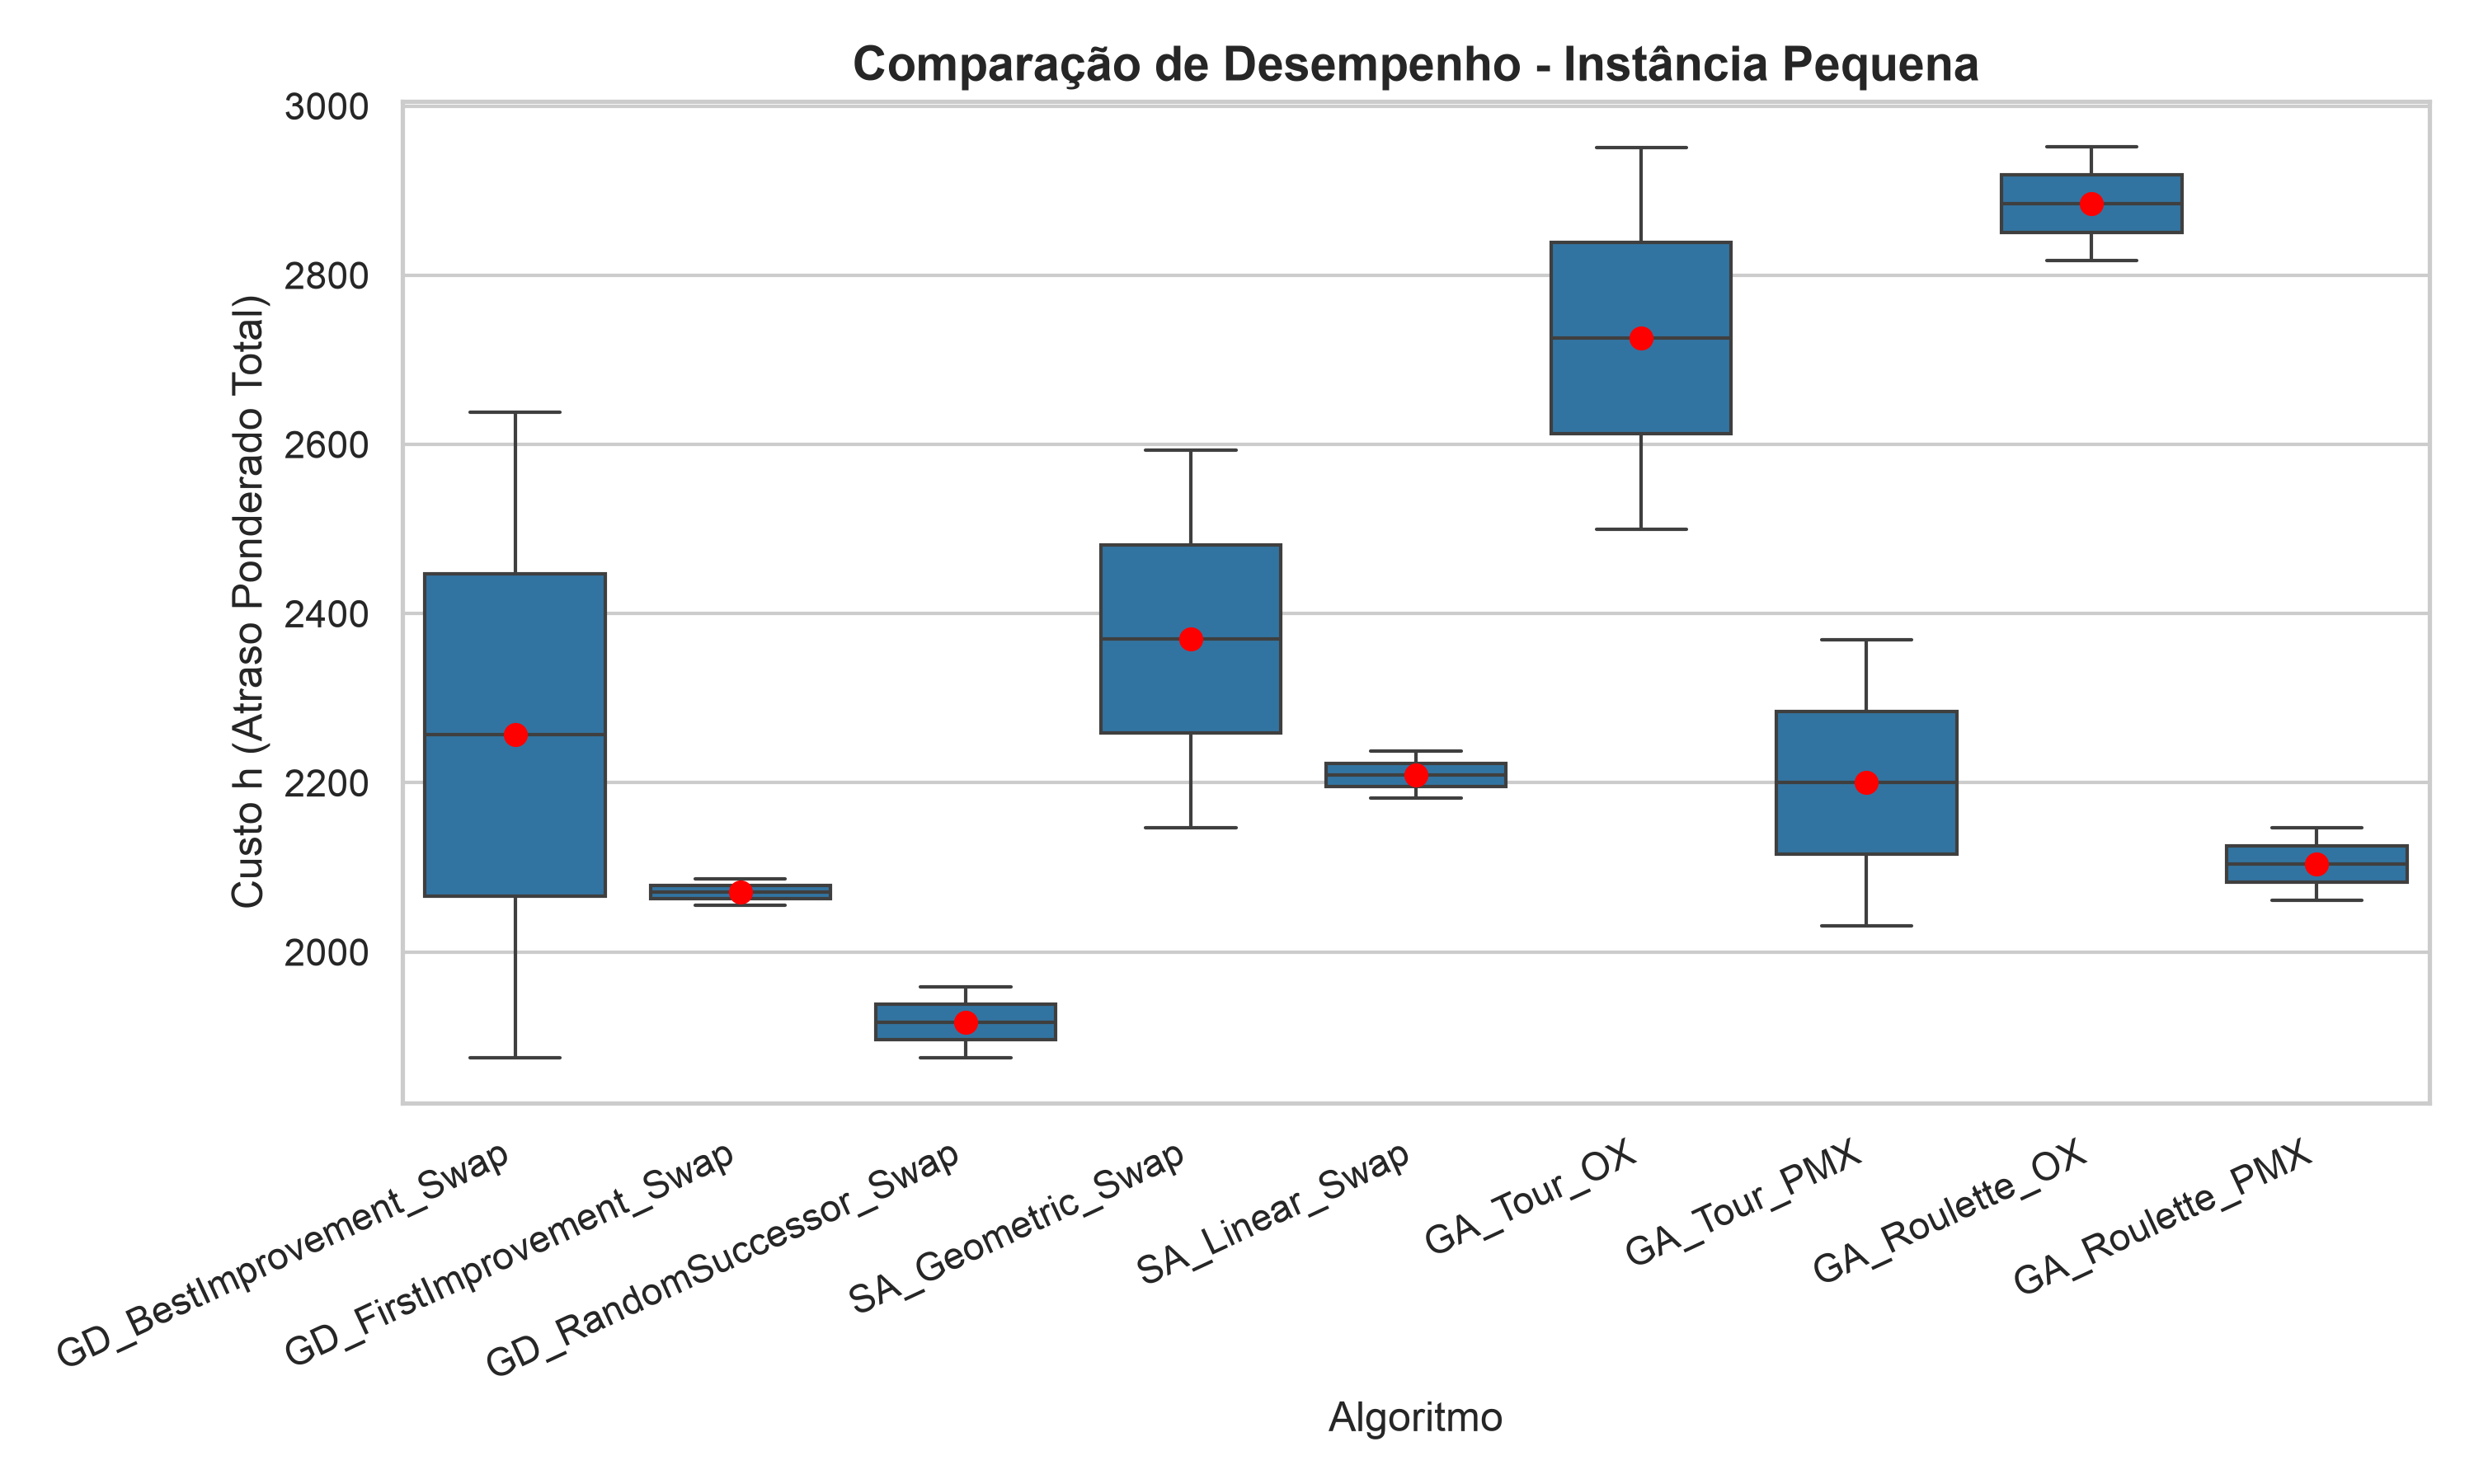
\includegraphics[width=\textwidth]{out/boxplot_pequena.png}
        \caption{Instância Pequena ($n=12$).}
    \end{subfigure}
    \hfill
    \begin{subfigure}[b]{0.32\textwidth}
        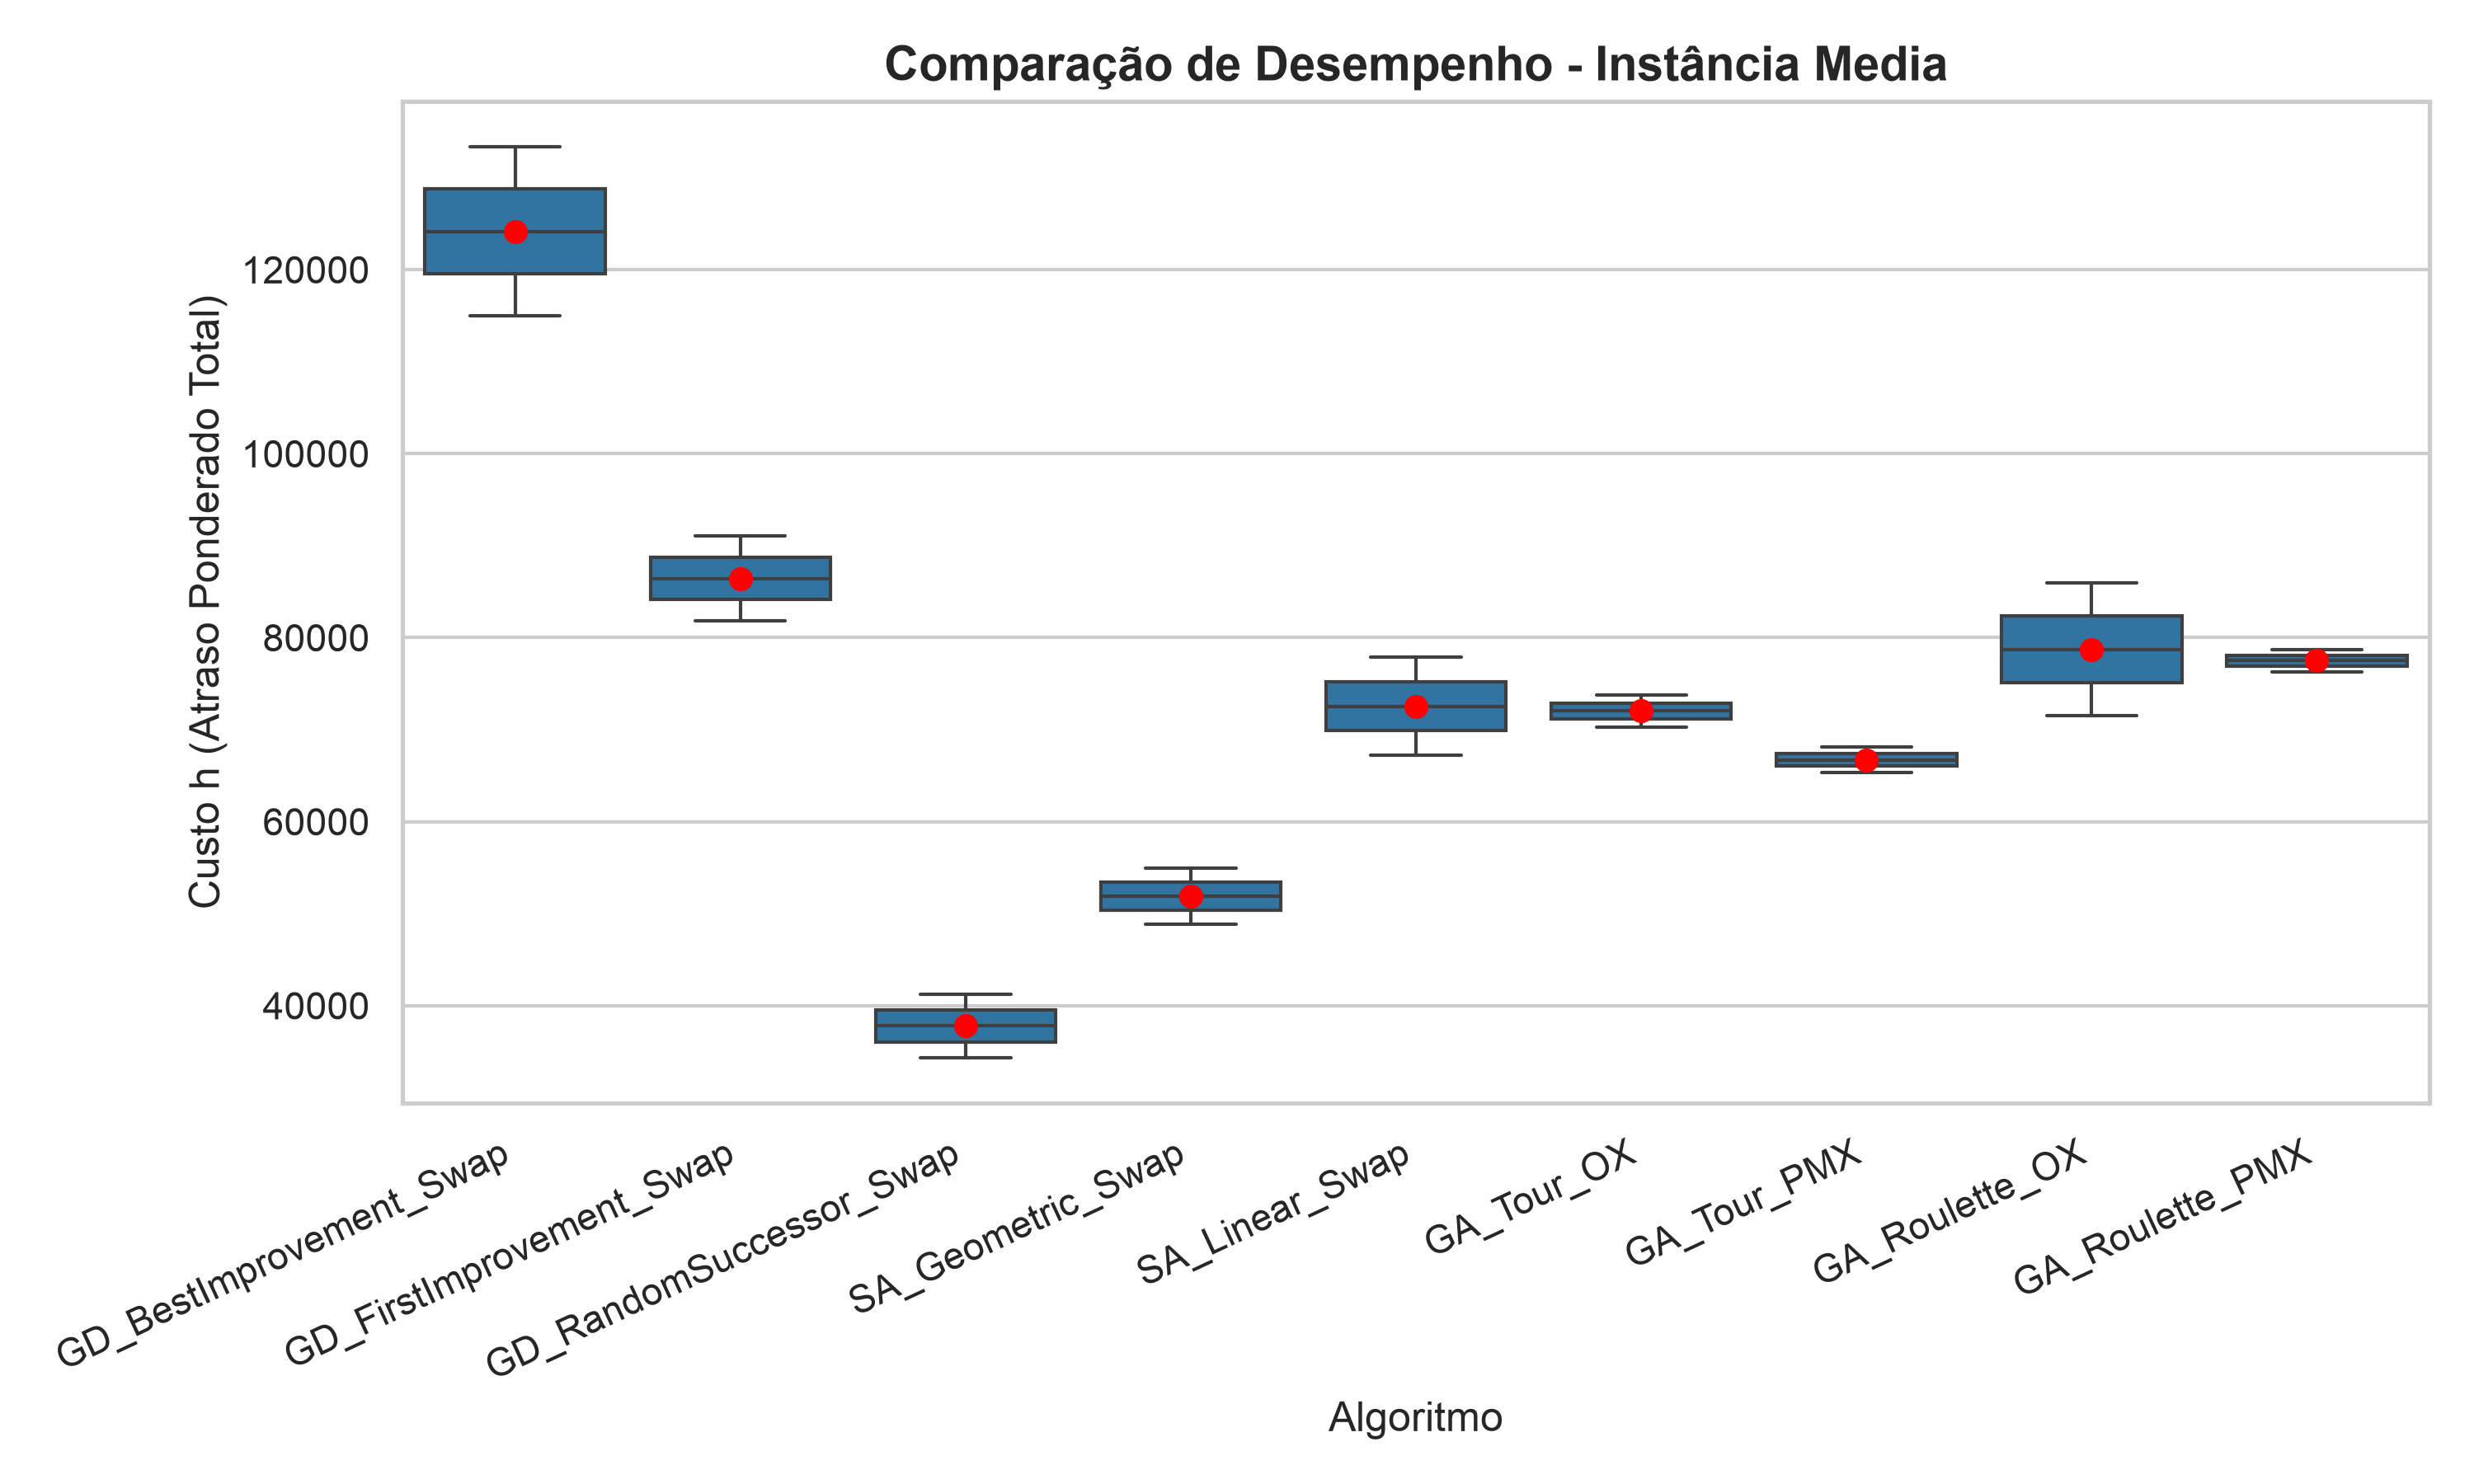
\includegraphics[width=\textwidth]{out/boxplot_media.png}
        \caption{Instância Média ($n=50$).}
    \end{subfigure}
    \hfill
    \begin{subfigure}[b]{0.32\textwidth}
        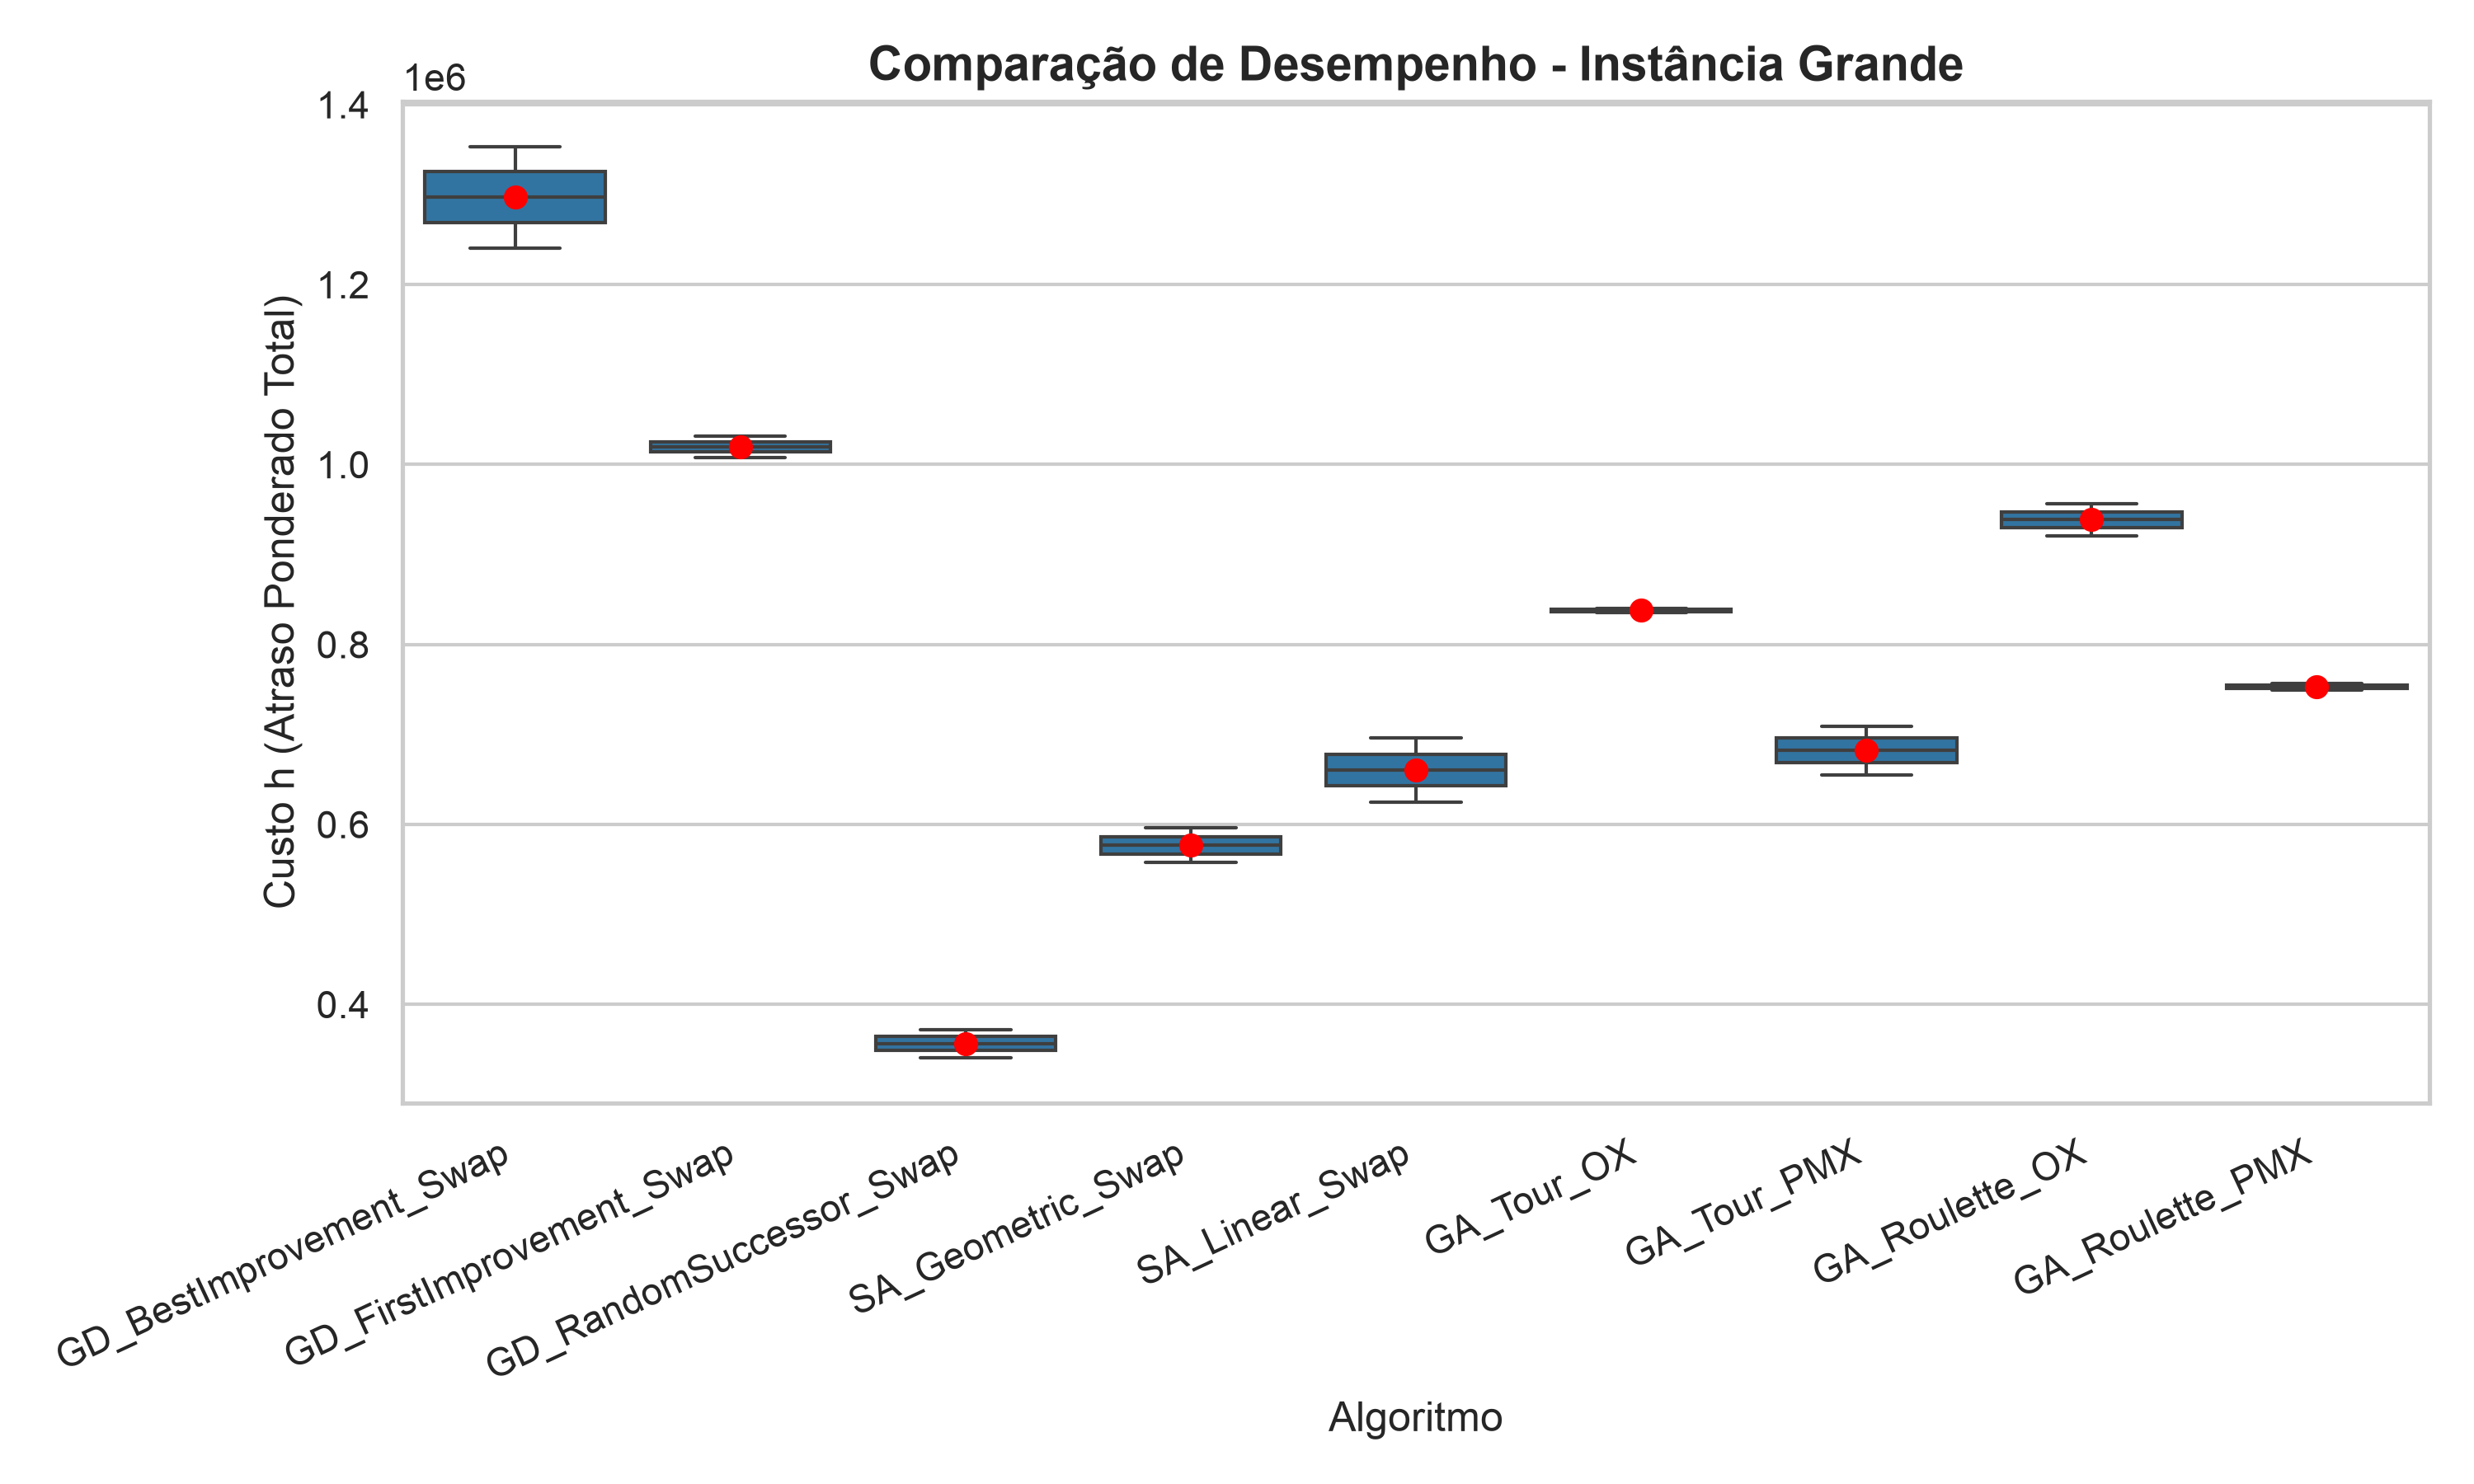
\includegraphics[width=\textwidth]{out/boxplot_grande.png}
        \caption{Instância Grande ($n=150$).}
    \end{subfigure}
    \caption{Boxplots comparativos do custo $h$ por instância.}
    \label{fig:boxplots}
\end{figure}

\begin{figure}[H]
    \centering
    \begin{subfigure}[b]{0.32\textwidth}
        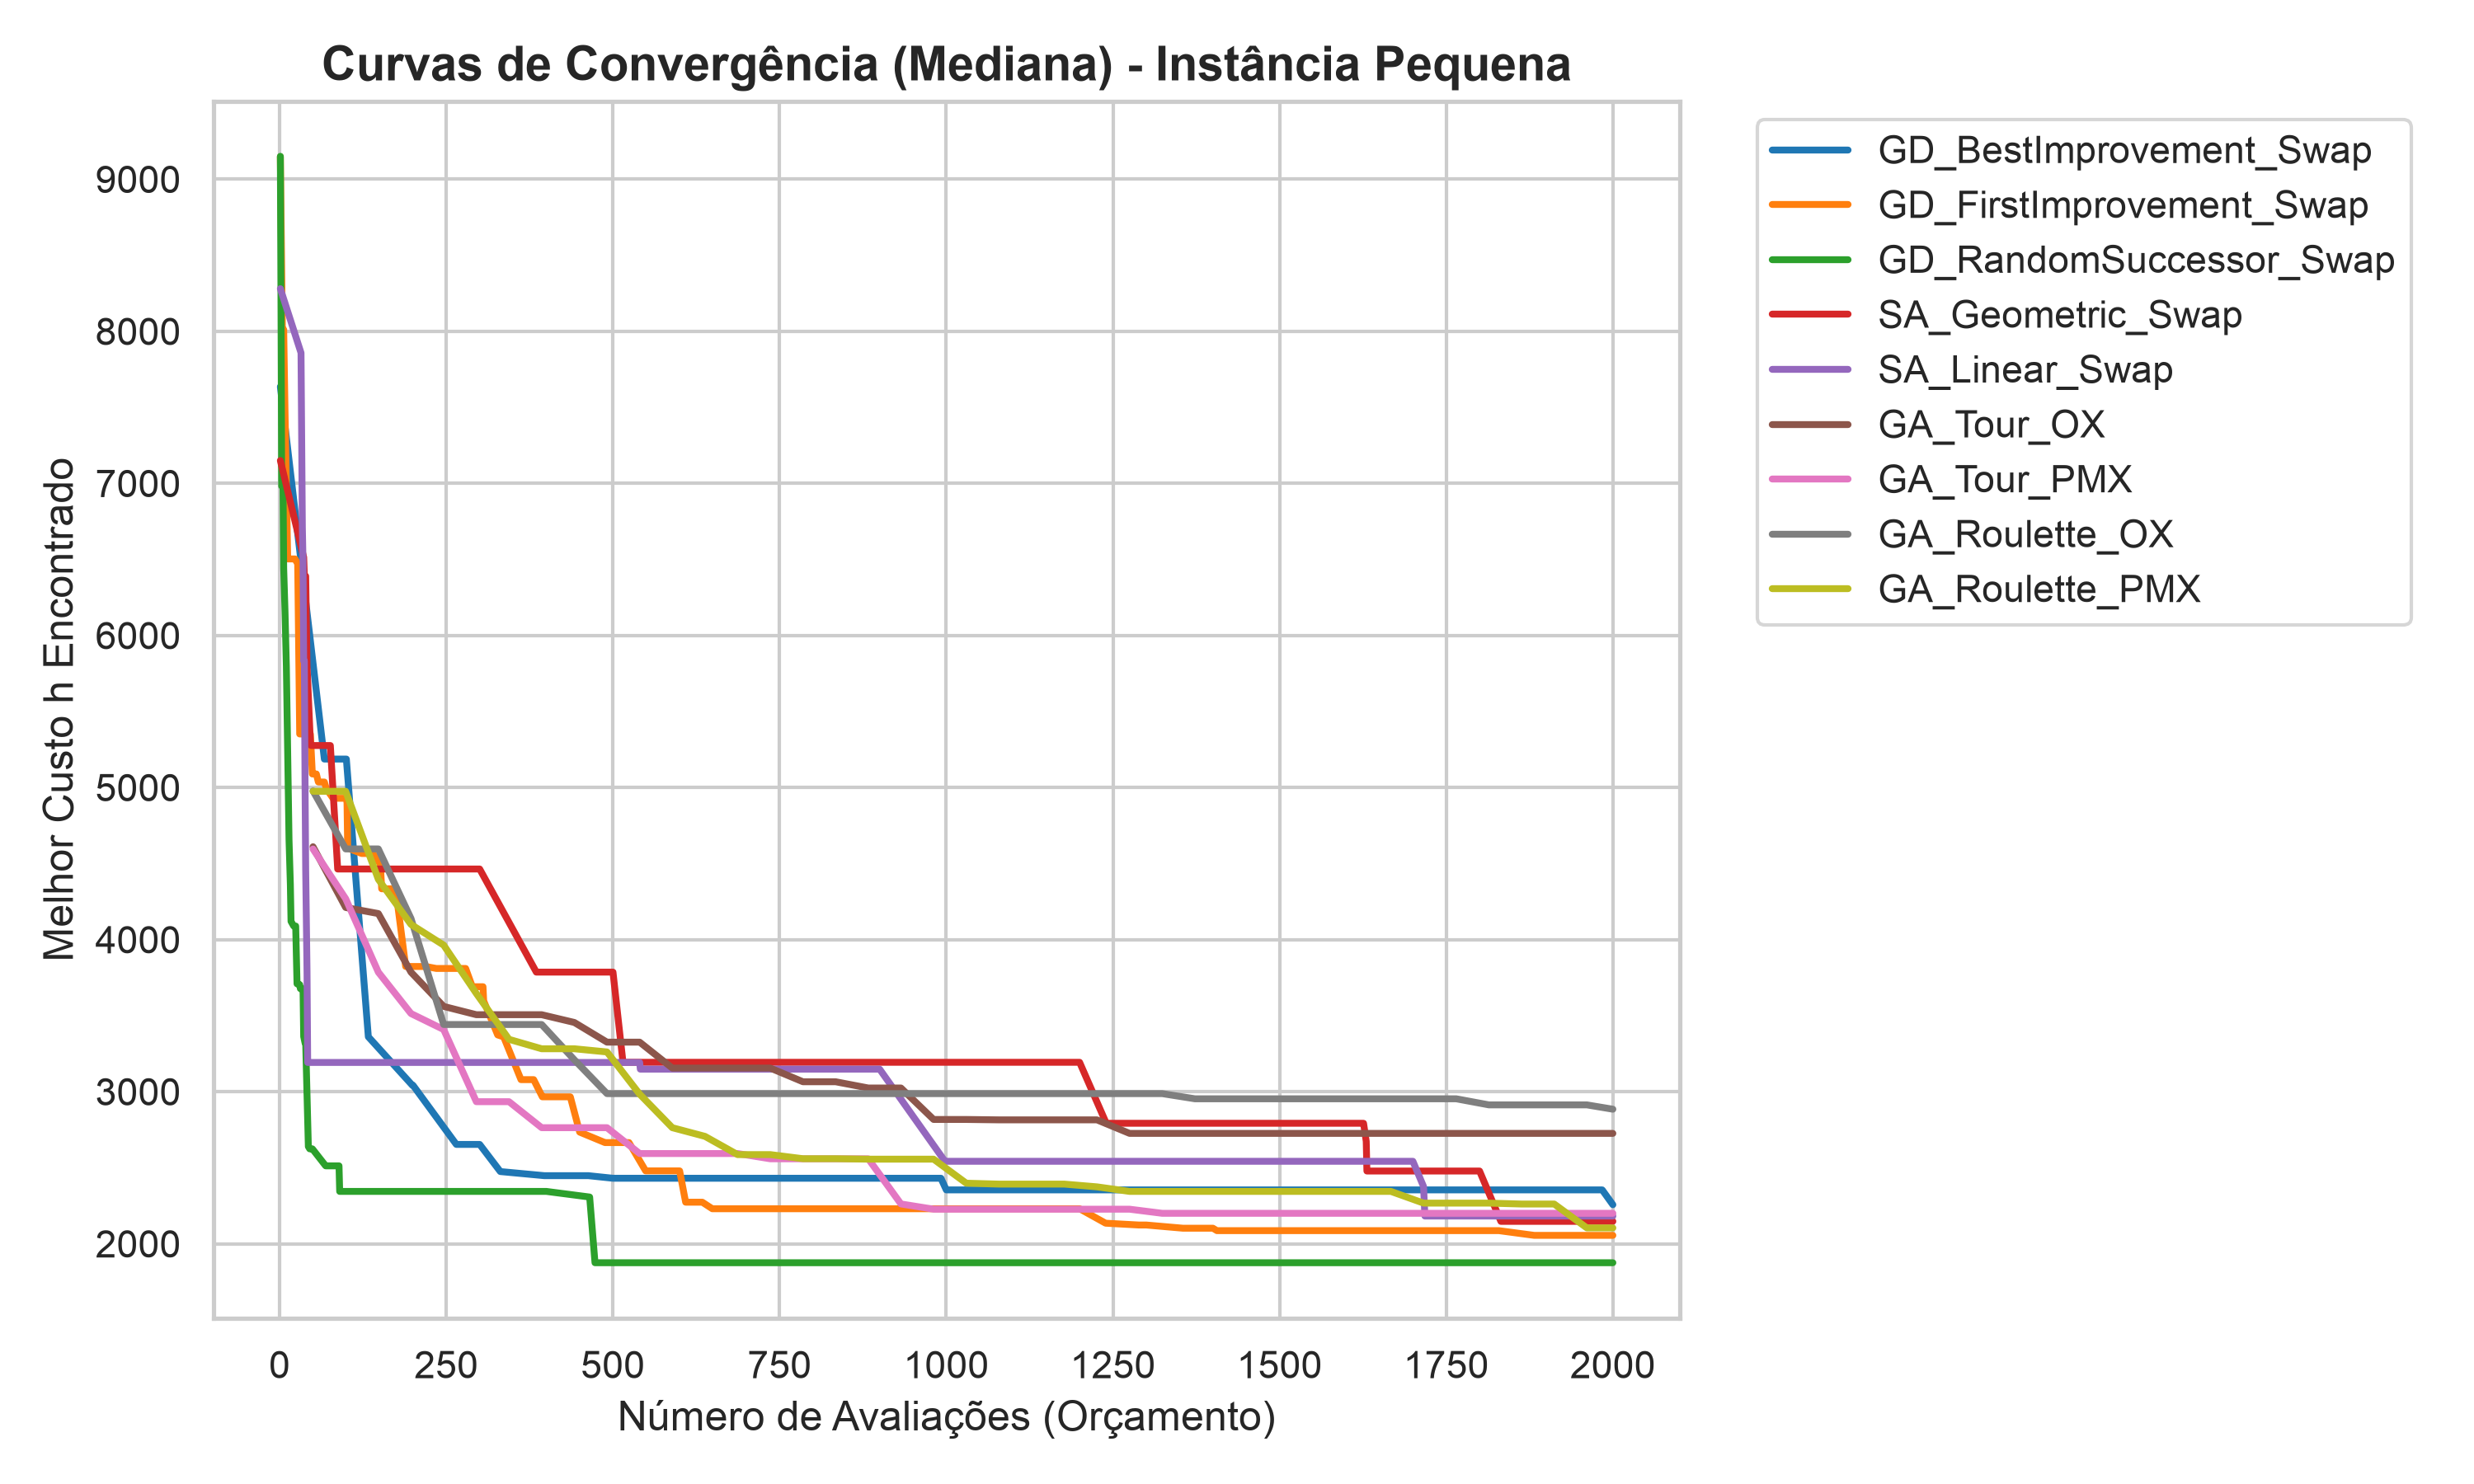
\includegraphics[width=\textwidth]{out/convergencia_pequena.png}
        \caption{Pequena ($n=12$).}
    \end{subfigure}
    \hfill
    \begin{subfigure}[b]{0.32\textwidth}
        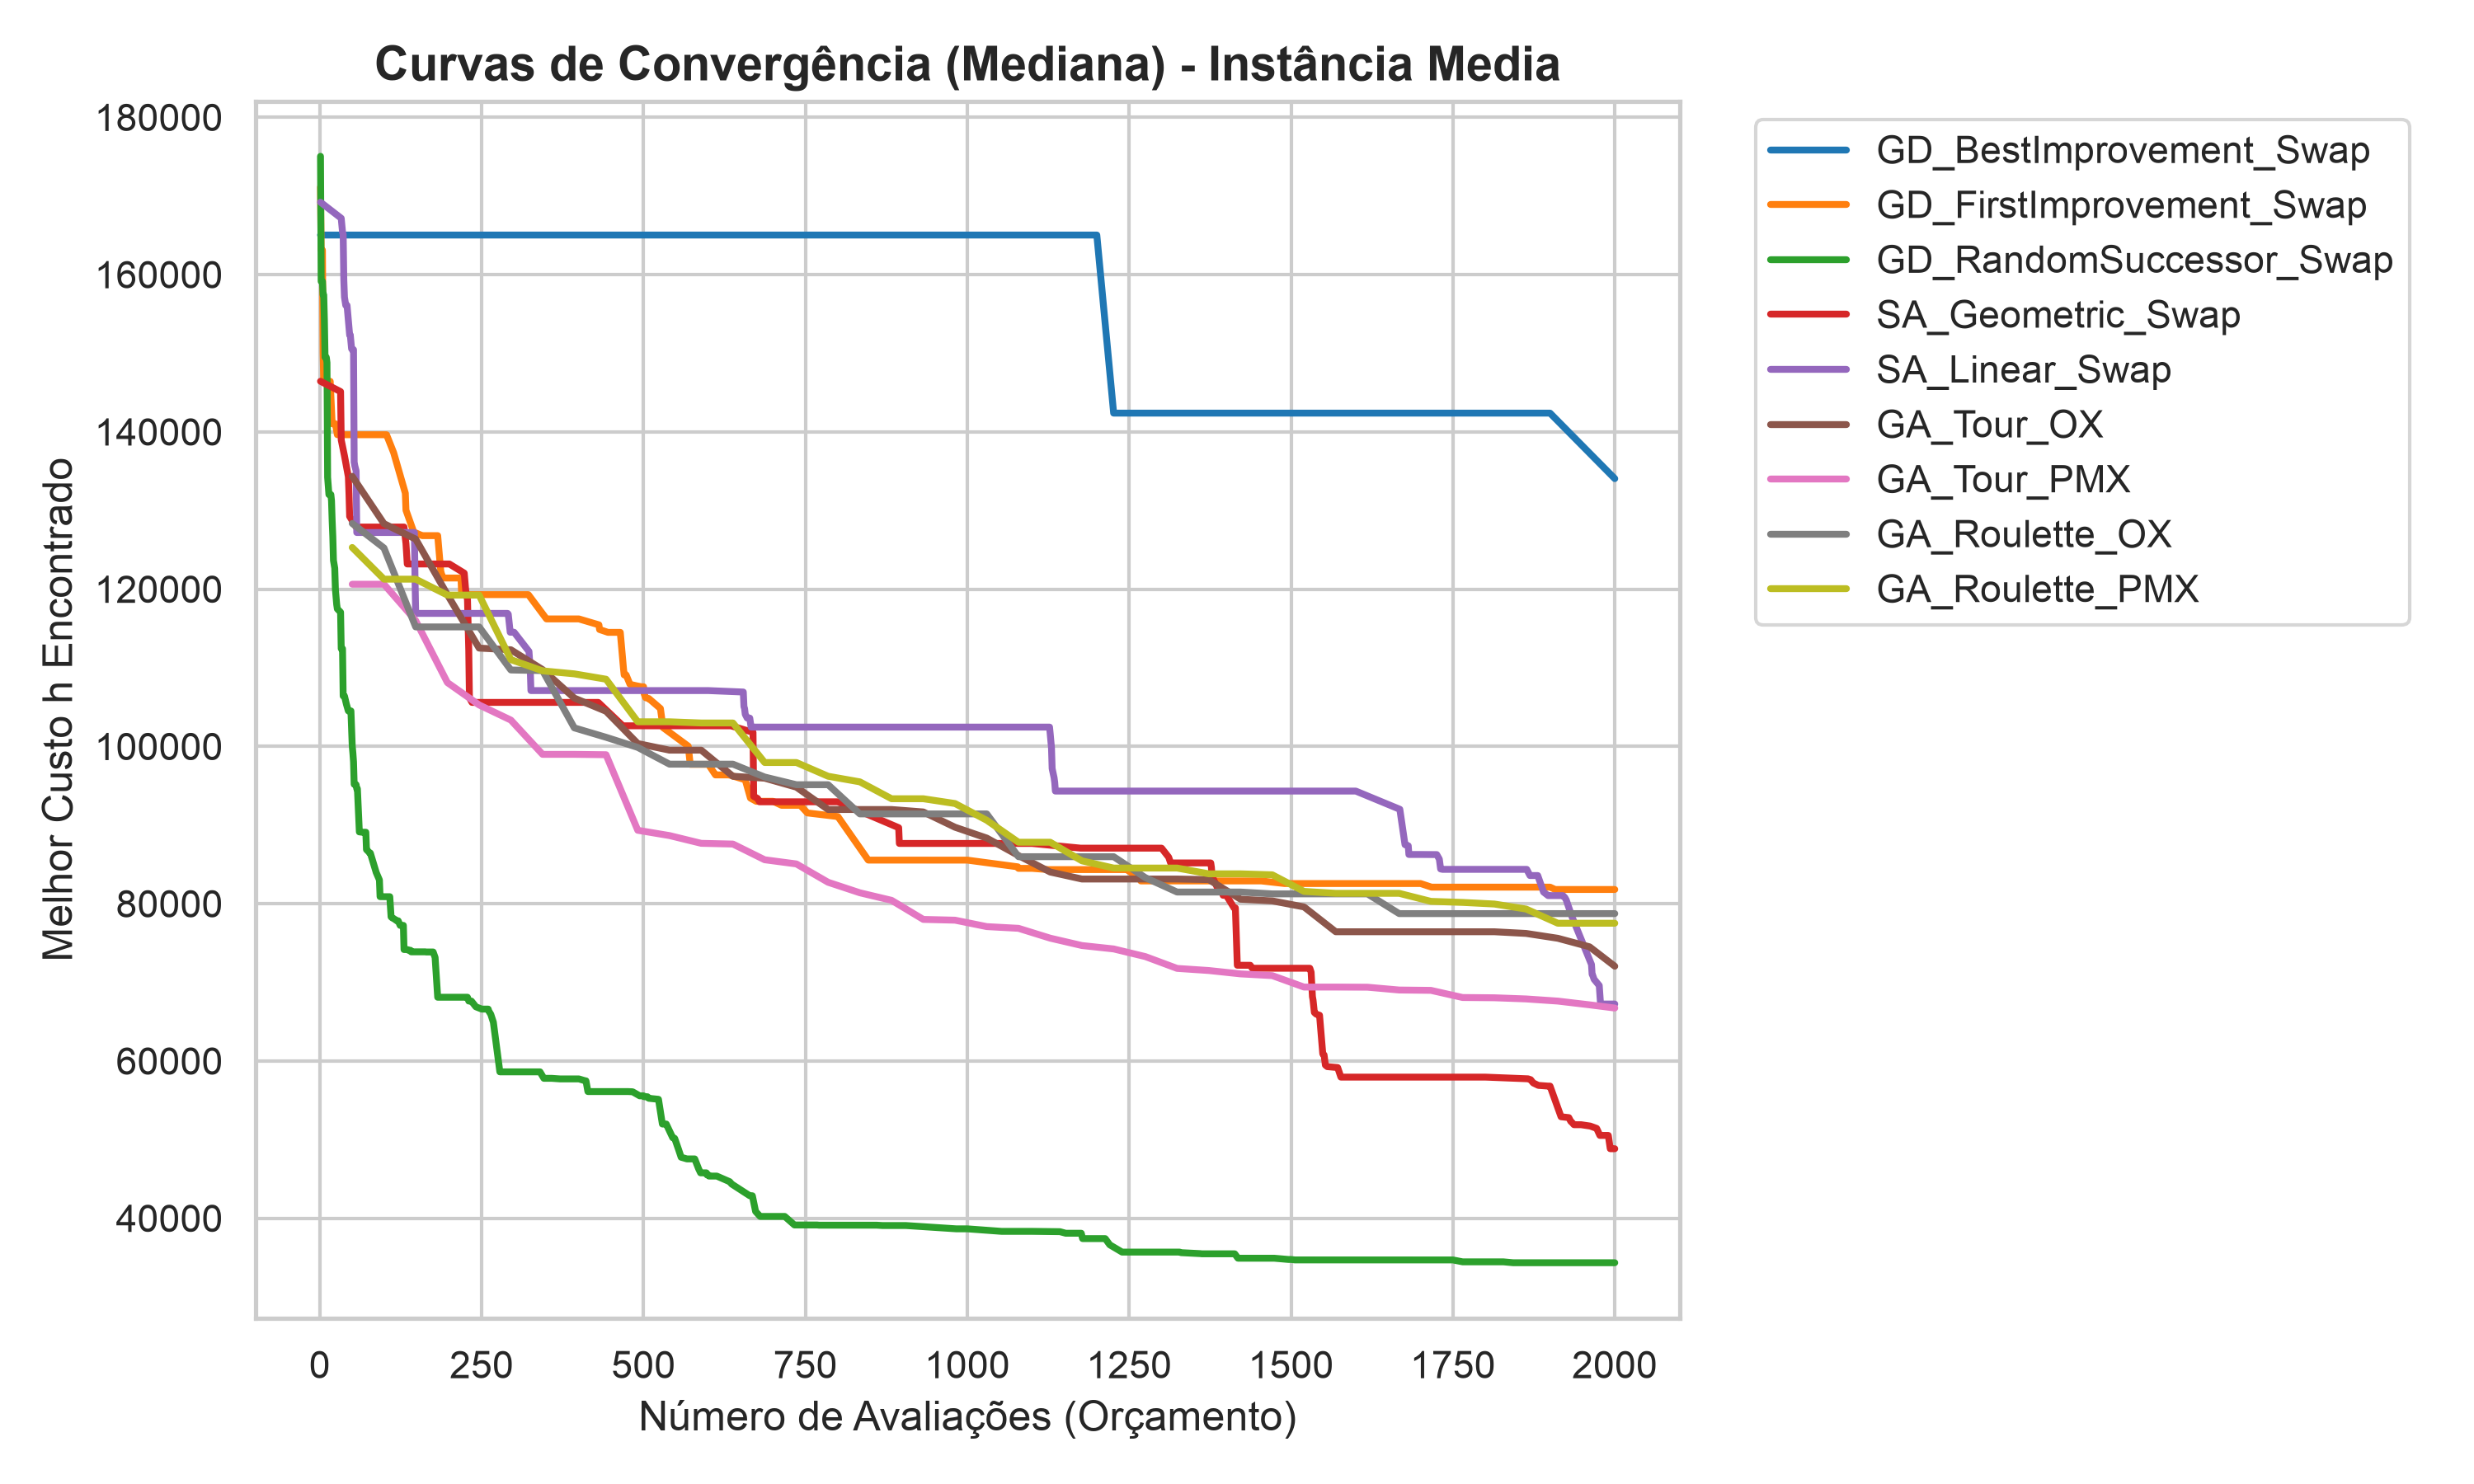
\includegraphics[width=\textwidth]{out/convergencia_media.png}
        \caption{Média ($n=50$).}
    \end{subfigure}
    \hfill
    \begin{subfigure}[b]{0.32\textwidth}
        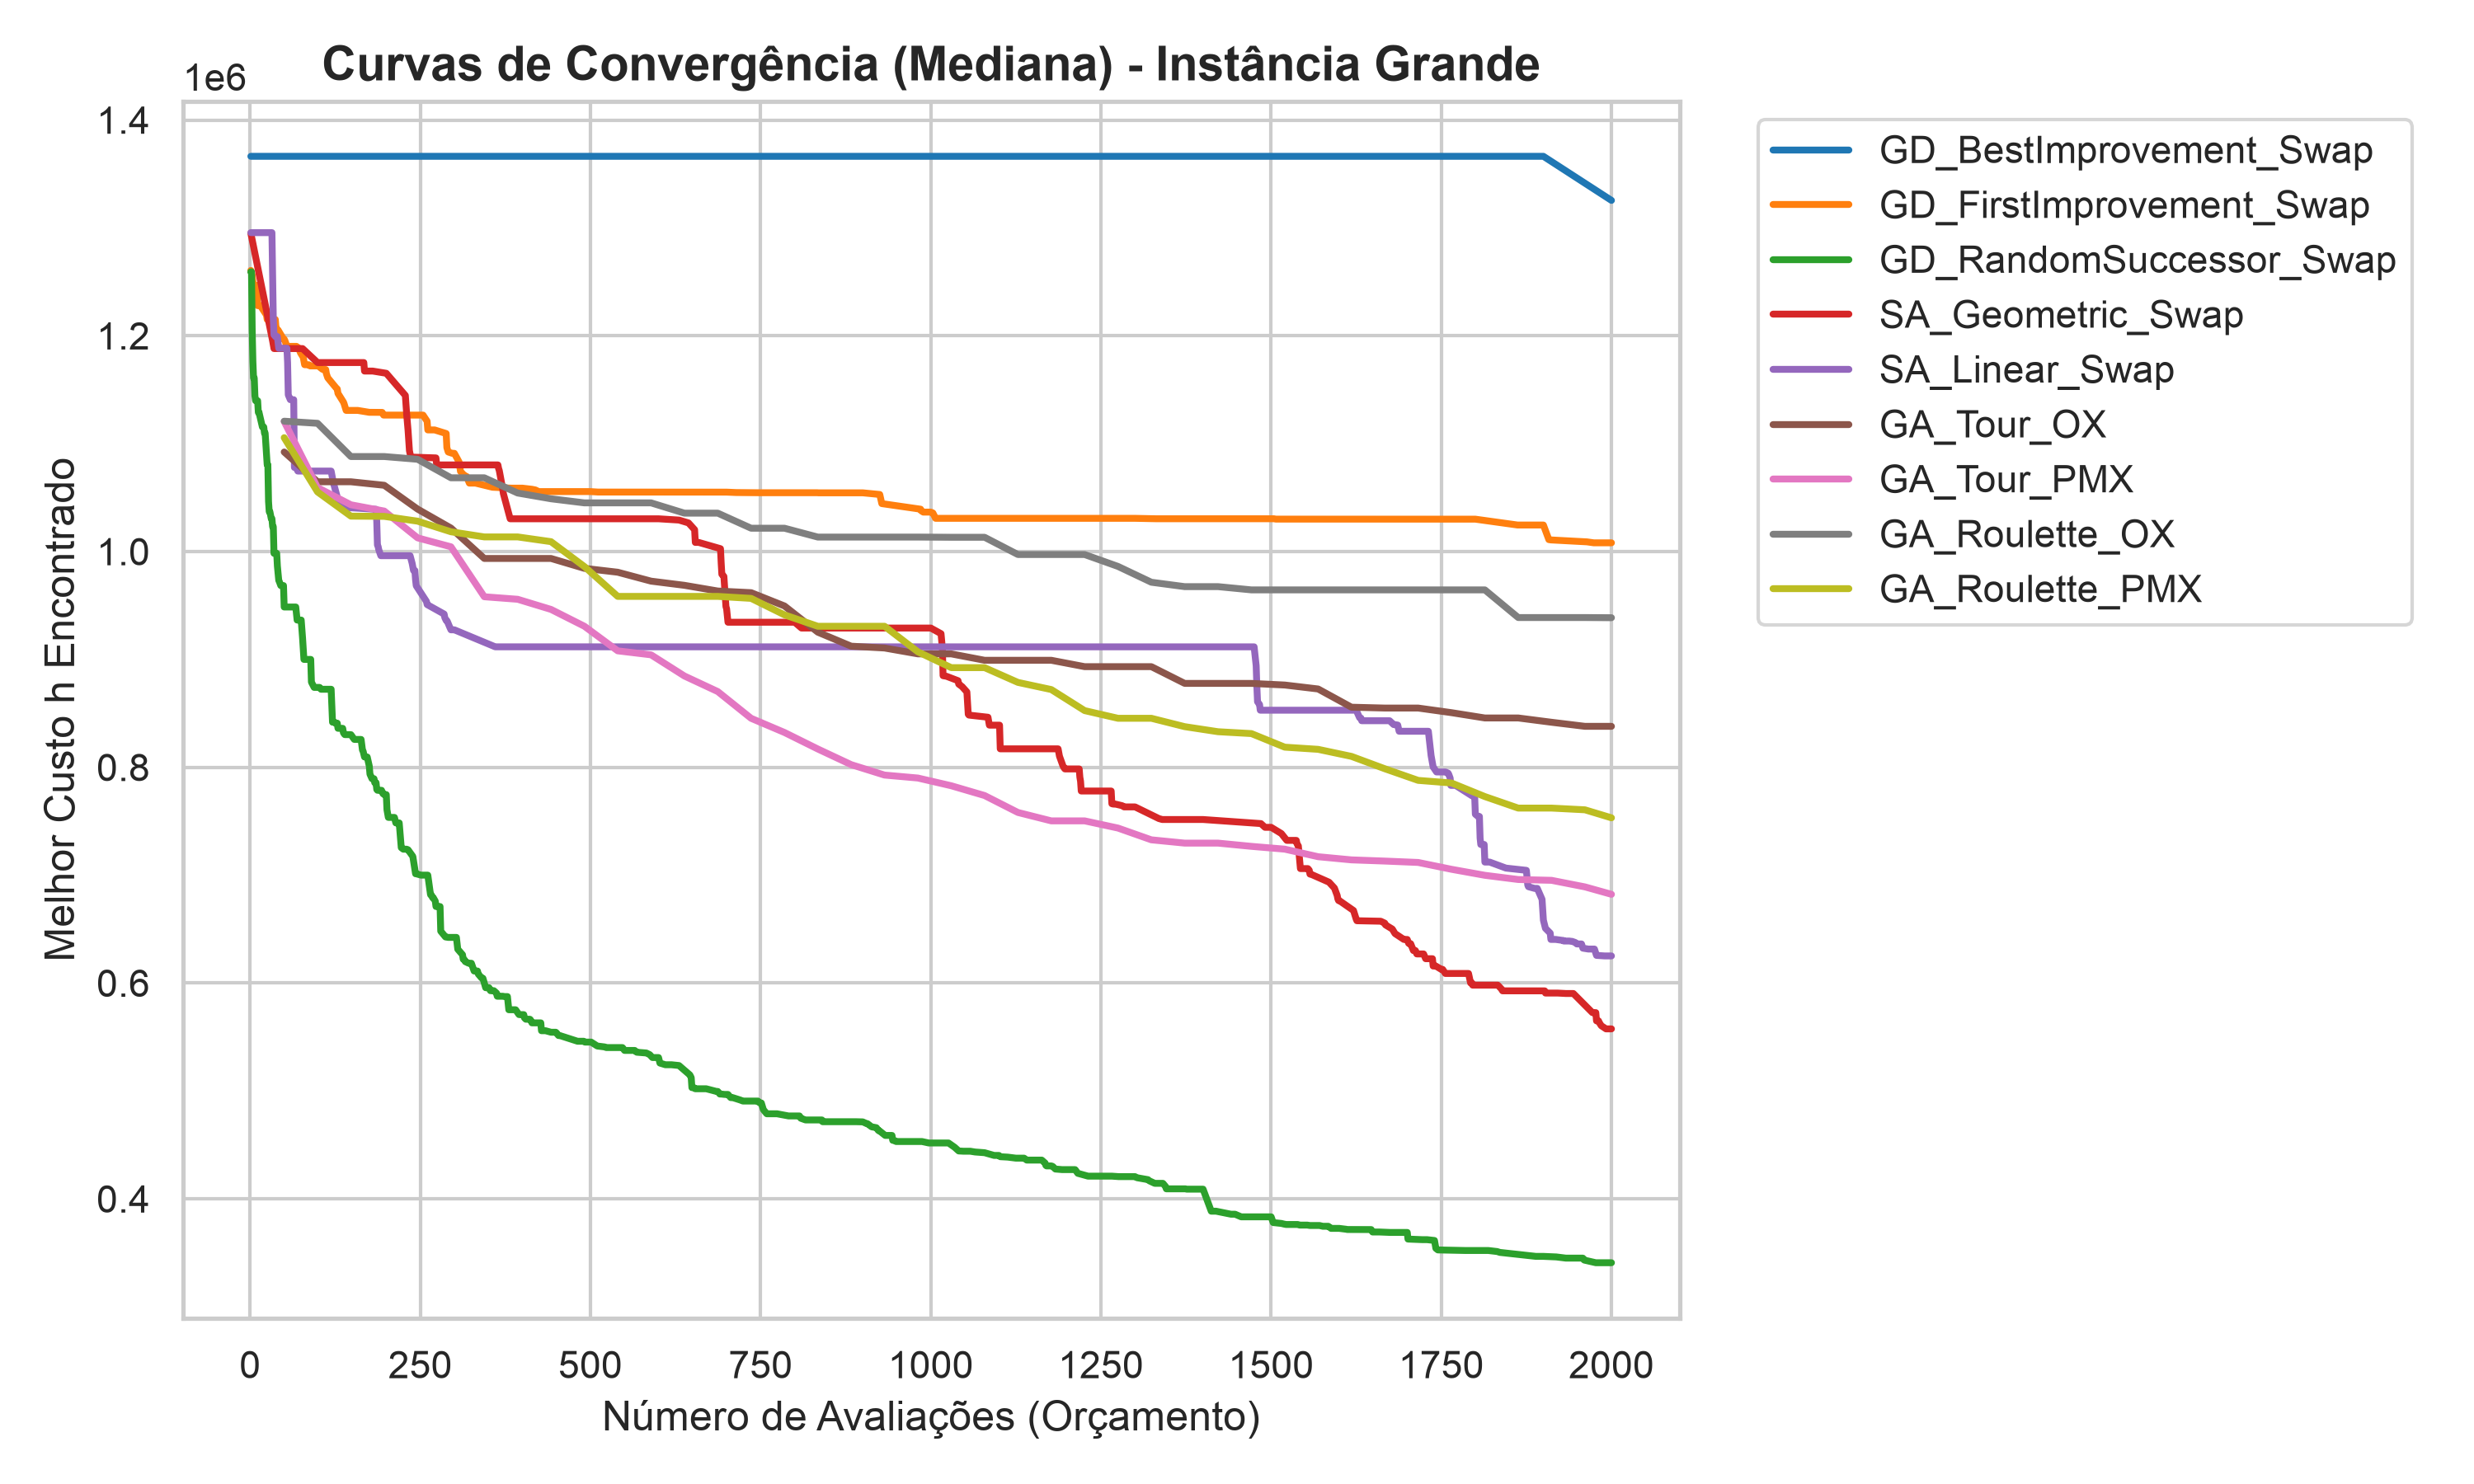
\includegraphics[width=\textwidth]{out/convergencia_grande.png}
        \caption{Grande ($n=150$).}
    \end{subfigure}
    \caption{Curvas de convergência mediana do melhor $h$ versus avaliações consumidas.}
    \label{fig:convergencia}
\end{figure}

\begin{figure}[H]
    \centering
    \begin{subfigure}[b]{0.48\textwidth}
        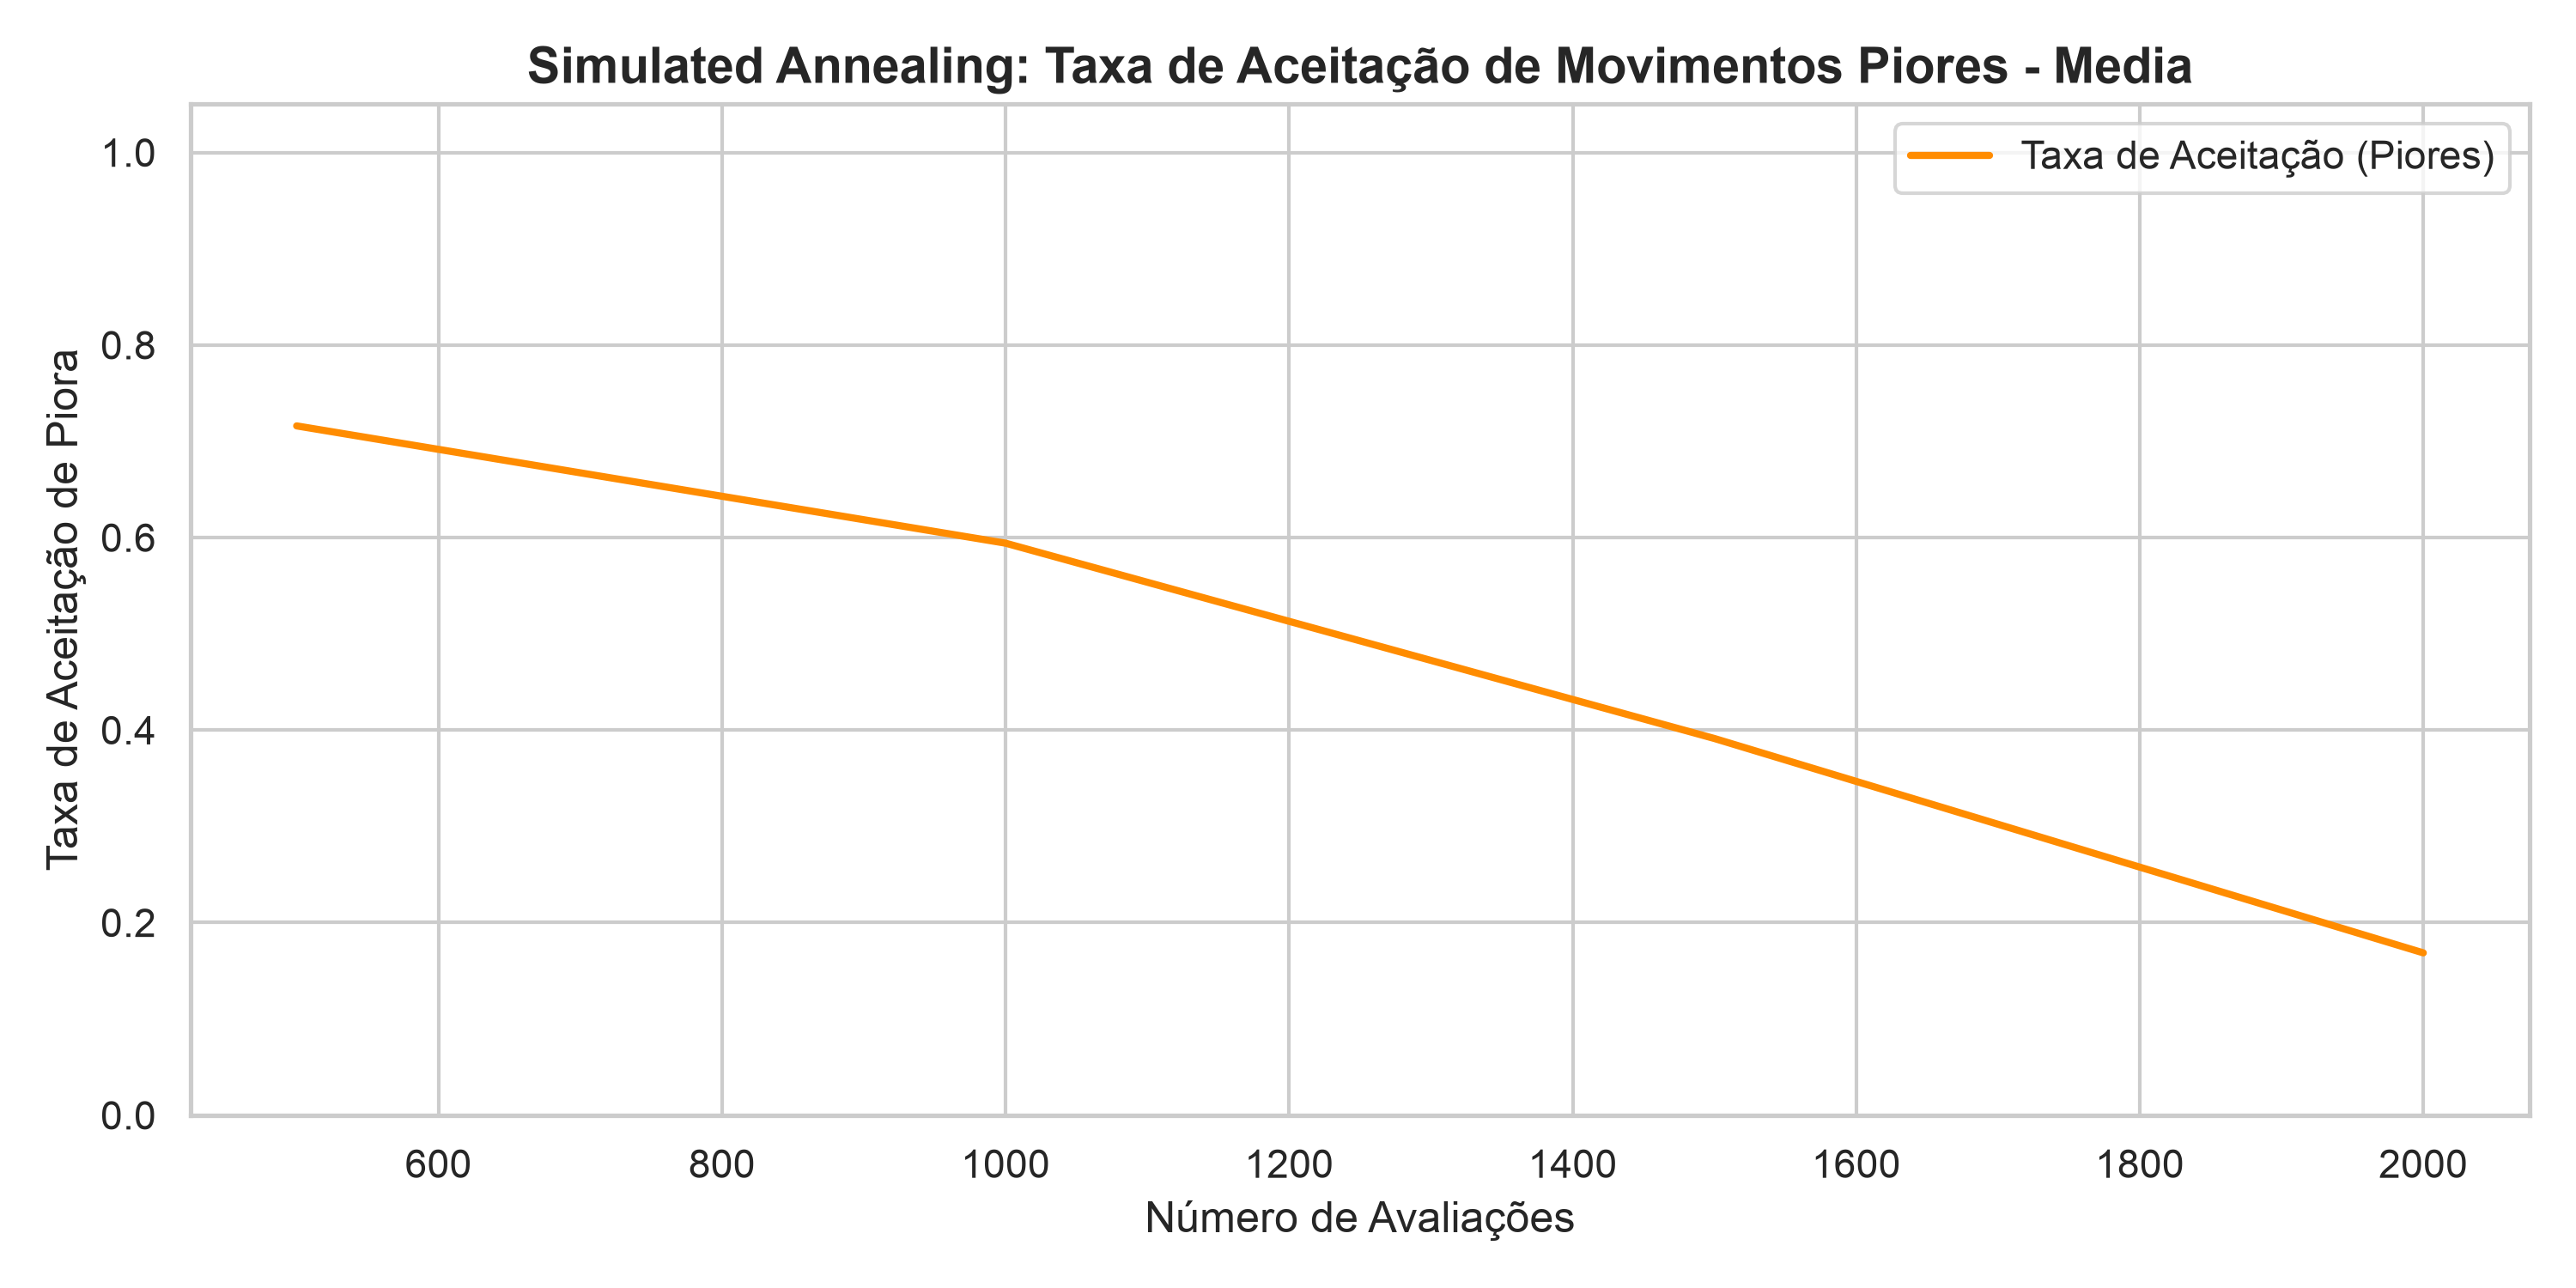
\includegraphics[width=\textwidth]{out/sa_aceitacao_media.png}
        \caption{Taxa de aceitação de movimentos piores no SA.}
        \label{fig:sa_acc}
    \end{subfigure}
    \hfill
    \begin{subfigure}[b]{0.48\textwidth}
        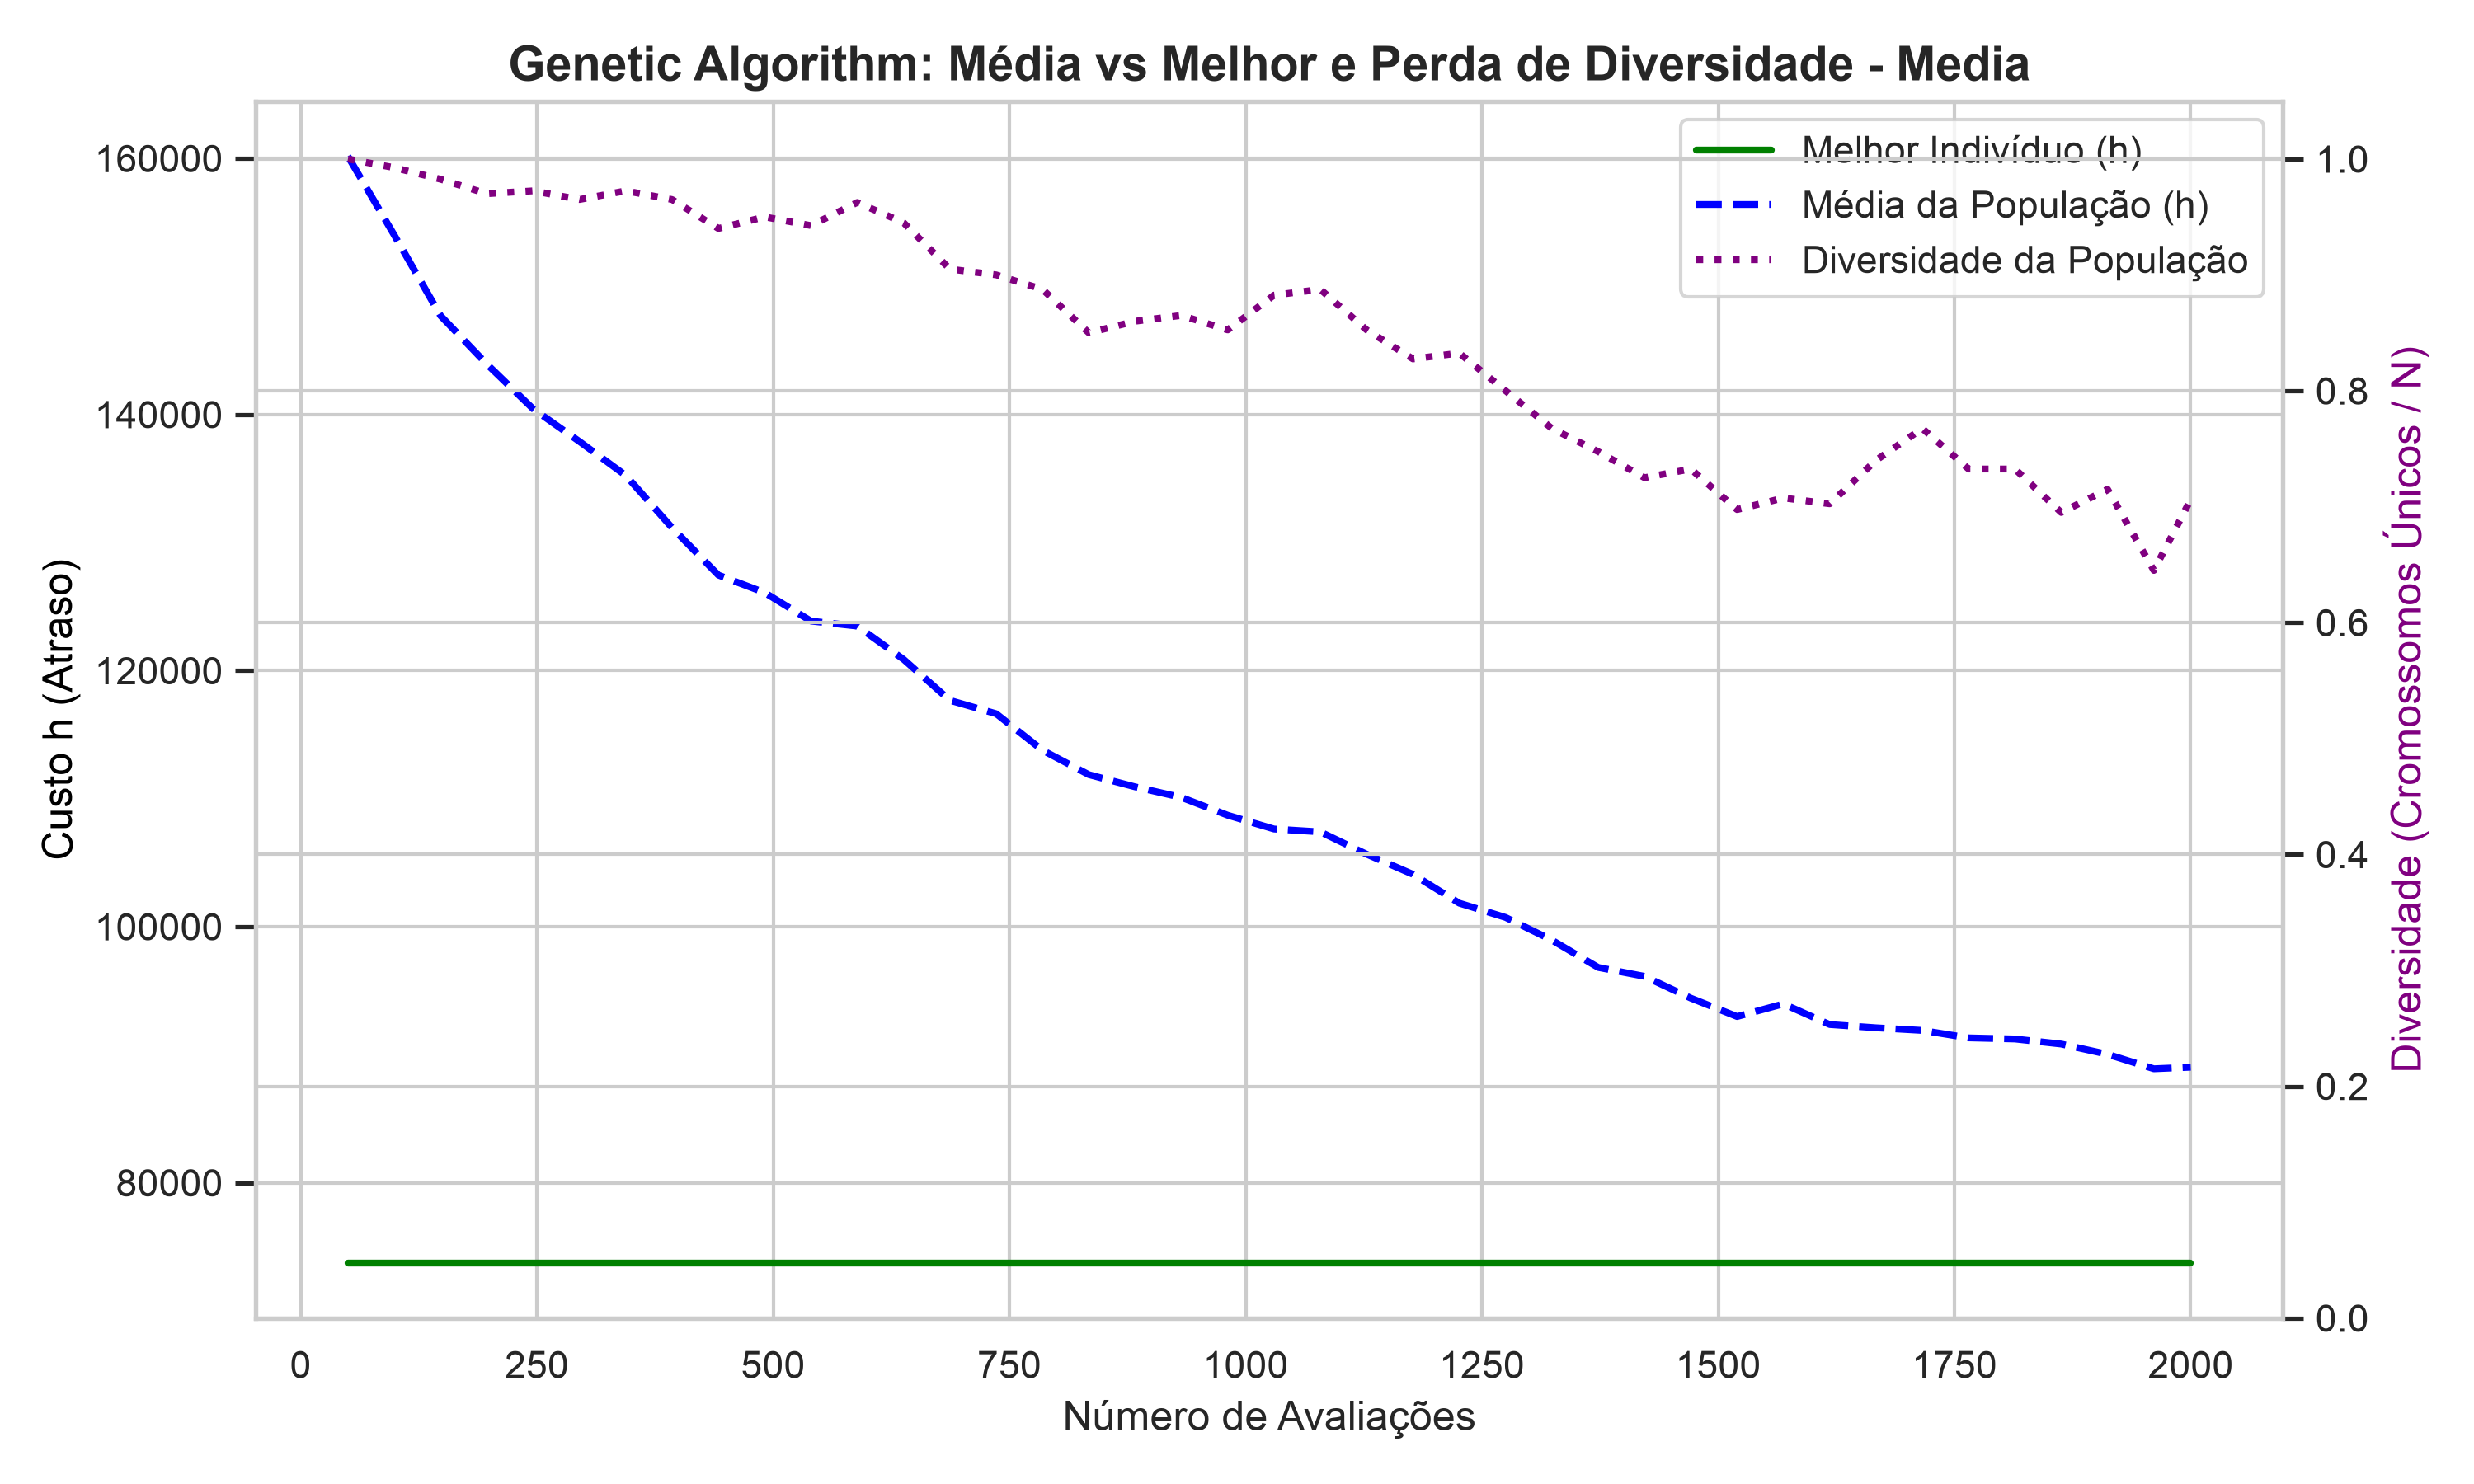
\includegraphics[width=\textwidth]{out/ga_diversidade_media.png}
        \caption{Média da população vs melhor indivíduo e diversidade no GA.}
        \label{fig:ga_div}
    \end{subfigure}
    \caption{Diagnóstico de comportamento interno dos algoritmos na instância média.}
\end{figure}

\section{Discussão Aprofundada dos Quatro Pontos Obrigatórios}

\subsection{1. Ótimos Locais e Random Restarts}
Na instância pequena ($n=12$, $V=66$), o espaço de estados contém bacias de atração relativamente pequenas. O \textbf{Greedy Descent com Random Restart} encontrou múltiplos ótimos locais distintos ao longo de suas execuções (uma média de 4 restarts no Best Improvement e 10 restarts no Random Successor). Em ambas as variantes estocásticas e de descida rápida, o algoritmo alcançou o ótimo global conhecido $h^* = 1875{,}0$ com frequência superior a $60\%$. 

Em contrapartida, conforme o tamanho da instância aumenta ($n=50$ e $n=150$), o Best Improvement deixa de realizar restarts: uma única varredura completa da vizinhança na instância grande já consome 11.175 avaliações. Como resultado, o Best Improvement realizou apenas 1 passo de melhoria e 0 restarts antes de esgotar o orçamento, ficando preso no primeiro platô local que encontrou.

\subsection{2. Equilíbrio entre Exploração e Intensificação}
\begin{itemize}
    \item \textbf{Greedy Descent:} É puramente intensificador durante a descida e puramente explorador no momento do \emph{random restart}. No entanto, quando $V(n)$ é astronômico, a intensificação consome todo o orçamento antes que a primeira bacia de atração seja concluída.
    \item \textbf{Simulated Annealing:} O mecanismo de exploração é regido pela probabilidade de Gibbs no início da busca (aceitando mais de $75\%$ das propostas de piora, como evidenciado na Figura~\ref{fig:sa_acc}). Conforme a temperatura decai, o algoritmo intensifica progressivamente na bacia mais promissora. O resfriamento geométrico superou o linear porque preserva mais tempo na faixa intermediária crítica de temperatura (\emph{critical temperature zone}), enquanto o linear esfria rápido demais no início e lento demais no fim.
    \item \textbf{Genetic Algorithm:} A recombinação e mutação atuam na exploração, enquanto o elitismo e a pressão de seleção (torneio) realizam a intensificação. A Figura~\ref{fig:ga_div} demonstra visualmente a perda de diversidade: nas gerações iniciais, a diversidade é próxima de 1{,}0; à medida que indivíduos dominantes se propagam, a população converge para um clone comum e a curva da média da população cola na curva do melhor indivíduo, tornando o GA ineficaz no terço final do orçamento.
\end{itemize}

\subsection{3. Efeito da Escala e Custo da Vizinhança}
O ranking dos algoritmos sofreu uma inversão radical da instância pequena para a grande:
\begin{itemize}
    \item Em $n=12$, o \textbf{GD Random Successor} e o \textbf{GD Best Improvement} empatam no topo ao atingir o ótimo global $h^*=1875$.
    \item Em $n=150$, o \textbf{GD Best Improvement} desaba para a pior colocação ($h > 1{,}2 \times 10^6$), enquanto o \textbf{GD Random Successor} atinge o melhor desempenho absoluto ($h \approx 356.425$), superando até mesmo o SA e o GA.
\end{itemize}
\textbf{Hipótese Teórica Confirmada:} Sob orçamento fixo de avaliações $B$, o custo de varredura do Best Improvement cresce quadraticamente com $O(n^2)$. Na instância grande, varrer uma única vizinhança custa $11.175$ avaliações, permitindo dar menos de 27 passos de descida em todo o orçamento. Já o \emph{Random Successor} aceita qualquer melhoria imediatamente ao custo de 1 avaliação, conseguindo dar mais de 200 passos de melhoria profundos no mesmo tempo.

\subsection{4. Quando o Algoritmo Genético Compensa?}
Em nenhuma das três instâncias o Algoritmo Genético superou a busca local estocástica (GD Random Successor e Simulated Annealing). 

\textbf{Hipótese Estrutural sobre a Codificação:} O problema de sequenciamento com atraso ponderado possui forte dependência posicional temporal contínua. Em uma rota $\pi$, o atraso de um ativo no fim da fila depende da soma de todos os tempos de trânsito anteriores. Ao realizar o crossover (seja OX ou PMX) entre dois pais de alta qualidade $\pi_A$ e $\pi_B$, que possuem blocos bons em posições temporais diferentes, a concatenação ou realocação desses blocos no filho desalinha os instantes de conclusão acumulados $C_k$, transformando ativos que estavam pontuais nos pais em tarefas com atrasos catastróficos no filho. Conclui-se que operadores de recombinação convencionais rompem a coerência cumulativa do prefixo, tornando a busca local em vizinhança uma abordagem estruturalmente superior para este problema.

\section{Conclusões}

Os experimentos comprovaram empiricamente que a superioridade de um algoritmo metaheurístico é indissociável da topologia do espaço de busca e da escala da vizinhança:
\begin{enumerate}
    \item A estratégia de \emph{Random Successor com Aceitação de Melhora} mostrou-se a mais eficiente e escalável sob orçamento limitado, superando a varredura exaustiva do \emph{Best Improvement}.
    \item O \emph{Simulated Annealing} apresentou excelente capacidade de escape de ótimos locais quando bem calibrado via resfriamento geométrico.
    \item A avaliação incremental e o desacoplamento de classes demonstraram ganhos de parede de $\approx 1{,}52\times$, confirmando o valor de uma arquitetura de software orientada a desempenho.
\end{enumerate}

\end{document}
